\section{Introduction \& Exact Pattern Matching}

% ── Section ──────────────────────────────────────────────
\subsection{Definition}

The exact pattern matching problem is defined as follows:
\begin{problem}[Exact pattern matching]
  Given an alphabet $\Sigma$, and two strings $T$, $P$ $\in \Sigma^*$, for which $|T| = n$ and $|P| = m$, find all
  occurrences of $P$ in $T$, i.e.\ compute $\{\, i \mid T[i,\, i+m-1] = P \,\}$.
\end{problem}

\subsubsection*{Notation}

Throughout these notes, $\Sigma$ denotes a finite alphabet of constant size ($|\Sigma| \in \Oh{1}$). For a string $S$ of length $|S|$:
\begin{itemize}[nosep]
  \item $S[i]$ denotes the $i$-th character of $S$ (1-based indexing).
  \item $S[i,j]$ denotes the substring $S[i]\,S[i+1]\cdots S[j]$ (empty string if $i > j$).
  \item $S[{,}j] = S[1,j]$ is the prefix of length $j$; $S[i{,}] = S[i,|S|]$ is the suffix starting at $i$.
\end{itemize}
A \emph{proper} prefix (resp.\ suffix) of $S$ is any prefix (resp.\ suffix) strictly shorter than $S$ itself.

\begin{example}
  Let $\Sigma = \{a, b\}$, $T = \texttt{ababbab}$ and $P = \texttt{abb}$. The only occurrence of $P$ in $T$ is at
  position $3$.
\end{example}

\subsection{Naive approach}
% ── Figure: naive matching ────────────────────────────────
\begin{figure}[H]
\centering
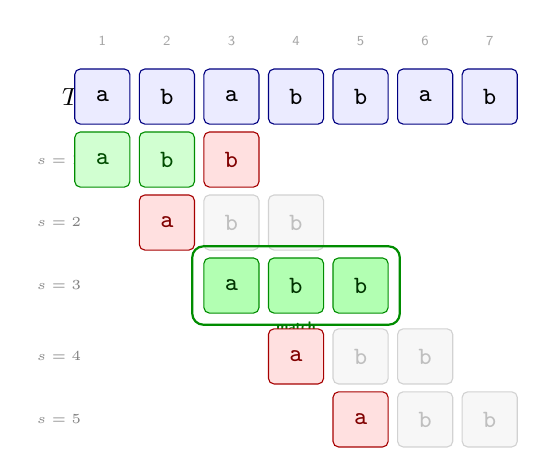
\begin{tikzpicture}[
  cell/.style={
    minimum width=7mm, minimum height=7mm,
    font=\ttfamily\small, inner sep=0pt,
    text centered, rounded corners=2pt,
  },
  Tcell/.style={cell, draw=blue!50!black, fill=blue!8},
  MC/.style={cell, draw=green!55!black, fill=green!18, text=green!30!black},
  XC/.style={cell, draw=red!65!black,   fill=red!12,   text=red!50!black},
  NC/.style={cell, draw=gray!35,        fill=gray!6,   text=gray!50},
  FM/.style={cell, draw=green!55!black, fill=green!30, text=green!20!black},
]

\def\cw{0.82}

% ── position indices (1-based) ───────────────────────────
\foreach \i in {1,...,7}
  \node[font=\tiny\sffamily, text=gray!70] at ({(\i-1)*\cw}, 1.9) {\i};

% ── T row ────────────────────────────────────────────────
\node[font=\small\ttfamily, anchor=east] at (-0.15, 1.2) {$T$};
\foreach \i/\c in {1/a, 2/b, 3/a, 4/b, 5/b, 6/a, 7/b}
  \node[Tcell] at ({(\i-1)*\cw}, 1.2) {\c};

% ── shift s=1 : P\kern0pt[1]=a✓ P\kern0pt[2]=b✓ P\kern0pt[3]=b✗ ────────────────
\node[font=\tiny\sffamily, text=gray] at (-0.55, 0.4) {$s=1$};
\node[MC] at (0*\cw, 0.4) {a};
\node[MC] at (1*\cw, 0.4) {b};
\node[XC] at (2*\cw, 0.4) {b};   % P\kern0pt[3]=b vs T\kern0pt[3]=a

% ── shift s=2 : P\kern0pt[1]=a✗ ─────────────────────────────────
\node[font=\tiny\sffamily, text=gray] at (-0.55, -0.4) {$s=2$};
\node[XC] at (1*\cw, -0.4) {a};  % P\kern0pt[1]=a vs T\kern0pt[2]=b
\node[NC] at (2*\cw, -0.4) {b};
\node[NC] at (3*\cw, -0.4) {b};

% ── shift s=3 : P\kern0pt[1]=a✓ P\kern0pt[2]=b✓ P\kern0pt[3]=b✓  →  MATCH ─────
\node[font=\tiny\sffamily, text=gray] at (-0.55, -1.2) {$s=3$};
\node[FM] (ma) at (2*\cw, -1.2) {a};
\node[FM] (mb) at (3*\cw, -1.2) {b};
\node[FM] (mc) at (4*\cw, -1.2) {b};
\draw[green!55!black, thick, rounded corners=4pt]
  ([xshift=-4pt, yshift=-4pt] ma.south west)
  rectangle
  ([xshift= 4pt, yshift= 4pt] mc.north east);
\node[font=\tiny\bfseries\sffamily, text=green!45!black]
  at (3*\cw, -1.72) {match};

% ── shift s=4 : P\kern0pt[1]=a✗ ─────────────────────────────────
\node[font=\tiny\sffamily, text=gray] at (-0.55, -2.1) {$s=4$};
\node[XC] at (3*\cw, -2.1) {a};  % P\kern0pt[1]=a vs T\kern0pt[4]=b
\node[NC] at (4*\cw, -2.1) {b};
\node[NC] at (5*\cw, -2.1) {b};

% ── shift s=5 : P\kern0pt[1]=a✗ ─────────────────────────────────
\node[font=\tiny\sffamily, text=gray] at (-0.55, -2.9) {$s=5$};
\node[XC] at (4*\cw, -2.9) {a};  % P\kern0pt[1]=a vs T\kern0pt[5]=b
\node[NC] at (5*\cw, -2.9) {b};
\node[NC] at (6*\cw, -2.9) {b};

\end{tikzpicture}
\caption{%
  Naive exact pattern matching of $P = \texttt{abb}$ in $T = \texttt{ababbab}$ (1-indexed).
  Each row corresponds to one shift $s$; the pattern $P$ is aligned starting at $T\kern0pt[s]$.
  \textcolor{green!45!black}{\textbf{Green}} = character matched,
  \textcolor{red!60!black}{\textbf{red}} = first mismatch (algorithm skips to next shift),
  \textcolor{gray}{gray} = not compared.
}
\label{fig:naive-matching}
\end{figure}


What the Figure \ref{fig:naive-matching} illustrates is one basic naive approach. In this approach we nest two loops: the outer loop iterates over all possible "first positions" $s$ in $T$ where the pattern $P$ could potentially match, and the inner loop checks character by character if $P$ matches $T$ starting from position $s$.
For example the first row of the figure corresponds to starting the search from index $s=1$ of $T$. Given $s$ we then loop one by one each character of $P$, moving along $T$ as well, and check if all the characters match. In this case we find a mismatch at the third character of $P$ (which is \texttt{b}, whereas the corresponding character in $T$ is \texttt{a}). When this happens, we break this inner loop and move to the next shift $s=2$.
If the length of the pattern was $m$ and the length of the text was $n$, the outer loop could have up to $\Oh{n}$ iterations, and each inner iteration could take up to $\Oh{m}$ time, leading to a worst-case time complexity of $\Oh{nm}$ for this naive approach.

% ── Figure: worst-case input ─────────────────────────────
\begin{figure}[H]
\centering
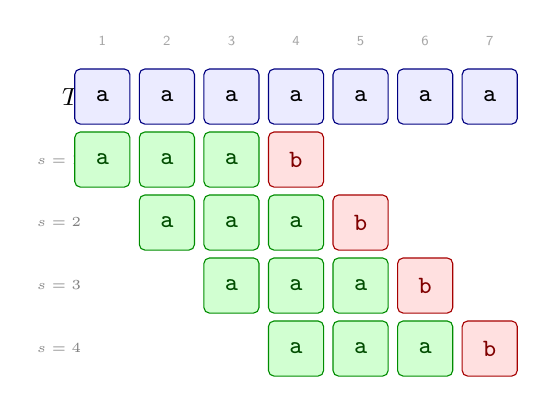
\begin{tikzpicture}[
  cell/.style={
    minimum width=7mm, minimum height=7mm,
    font=\ttfamily\small, inner sep=0pt,
    text centered, rounded corners=2pt,
  },
  Tcell/.style={cell, draw=blue!50!black, fill=blue!8},
  MC/.style={cell, draw=green!55!black, fill=green!18, text=green!30!black},
  XC/.style={cell, draw=red!65!black,   fill=red!12,   text=red!50!black},
]

% T = aaaaaaa (n=7),  P = aaab (m=4)
% every shift does m-1 = 3 matches before hitting b vs a

\def\cw{0.82}

% position indices (1-based)
\foreach \i in {1,...,7}
  \node[font=\tiny\sffamily, text=gray!70] at ({(\i-1)*\cw}, 1.9) {\i};

% T row
\node[font=\small\ttfamily, anchor=east] at (-0.15, 1.2) {$T$};
\foreach \i in {1,...,7}
  \node[Tcell] at ({(\i-1)*\cw}, 1.2) {a};

% s=1 : a✓ a✓ a✓ b✗
\node[font=\tiny\sffamily, text=gray] at (-0.55,  0.4) {$s=1$};
\node[MC] at (0*\cw,  0.4) {a};
\node[MC] at (1*\cw,  0.4) {a};
\node[MC] at (2*\cw,  0.4) {a};
\node[XC] at (3*\cw,  0.4) {b};

% s=2 : a✓ a✓ a✓ b✗
\node[font=\tiny\sffamily, text=gray] at (-0.55, -0.4) {$s=2$};
\node[MC] at (1*\cw, -0.4) {a};
\node[MC] at (2*\cw, -0.4) {a};
\node[MC] at (3*\cw, -0.4) {a};
\node[XC] at (4*\cw, -0.4) {b};

% s=3 : a✓ a✓ a✓ b✗
\node[font=\tiny\sffamily, text=gray] at (-0.55, -1.2) {$s=3$};
\node[MC] at (2*\cw, -1.2) {a};
\node[MC] at (3*\cw, -1.2) {a};
\node[MC] at (4*\cw, -1.2) {a};
\node[XC] at (5*\cw, -1.2) {b};

% s=4 : a✓ a✓ a✓ b✗
\node[font=\tiny\sffamily, text=gray] at (-0.55, -2.0) {$s=4$};
\node[MC] at (3*\cw, -2.0) {a};
\node[MC] at (4*\cw, -2.0) {a};
\node[MC] at (5*\cw, -2.0) {a};
\node[XC] at (6*\cw, -2.0) {b};

\end{tikzpicture}
\caption{%
  Worst-case input for the naive algorithm: $T = \texttt{aaaaaaa}$ ($n=7$) and
  $P = \texttt{aaab}$ ($m=4$).
  Every shift $s$ performs $m-1$ successful comparisons before the inevitable
  mismatch on $P\kern0pt[m] = \texttt{b}$, giving $(n-m+1)(m-1) = \Th{nm}$ total comparisons.
}
\label{fig:naive-worst-case}
\end{figure}
In figure \ref{fig:naive-worst-case} we see an example of a worst-case input for the naive algorithm.
In this case the text $T$ consists of $n$ \texttt{a} characters, and the pattern $P$ consists of $m-1$ \texttt{a} characters followed by a \texttt{b}.
There are $n-m+1$ possible shifts $s$ where the pattern could potentially match, and for each of these shifts the algorithm will successfully match the first $m-1$ characters of $P$. In the example of the figure we have $n=7$ and $m=4$, so there are $7-4+1=4$ shifts to check, and for each shift we make $m$ checks, of which $m-1=3$ are successful matches before we encounter the mismatch at the last character of $P$.
This results in a total of $(n-m+1)(m-1)$ comparisons, which is $\Theta(nm)$ in the worst case.

\begin{algorithm}[H]
  \caption{Naive exact pattern matching}
  \KwIn{Text $T[1\ldots n]$, Pattern $P[1\ldots m]$}
  \KwOut{All positions $s$ such that $T[s,s+m-1] = P$}
  \For{$s \gets 1$ \KwTo $n - m + 1$}{
    $j \gets 1$ \;
    \While{$j \leq m$ \textbf{and} $T[s+j-1] = P\kern0pt[j]$}{
      $j \gets j + 1$ \;
    }
    \If{$j > m$}{
      \textbf{output} $s$ \;
    }
  }
\end{algorithm}

\subsubsection{Correctness}

To pin down what ``the inner loop does'' precisely, let's give a name to the obvious quantity: for any position $i$ in $T$, write
\[
  \mathrm{common}(i) \;=\; \max\bigl\{\, k \geq 0 \mid T[i, i+k-1] = P[1,k] \,\bigr\}
\]
for the length of the longest common prefix of $T[i{,}]$ and $P$ — basically, how many characters of $P$ would match if you aligned it at position $i$.

\begin{lemma}
  \label{lem:naive-inner}
  At shift $s$, the inner loop exits with $j = \mathrm{common}(s) + 1$.
\end{lemma}
\begin{proof}
  Track the invariant: entering each iteration, we have $T[s, s+j-2] = P[1, j-1]$
  (the first $j-1$ characters already matched).  The loop keeps going as long as
  the next character also matches; it stops the moment it doesn't, or when $j$
  runs past $m$.  Since $\mathrm{common}(s)$ is exactly how many consecutive
  characters agree, the loop stops right at $j = \mathrm{common}(s)+1$.
\end{proof}

\begin{theorem}
  The naive algorithm finds every occurrence of $P$ in $T$, and nothing more.
\end{theorem}
\begin{proof}
  The outer loop visits every shift $s \in \{1, \ldots, n-m+1\}$, so no candidate
  starting position is ever skipped.  By Lemma~\ref{lem:naive-inner}, after the
  inner loop we have $j = \mathrm{common}(s)+1$; the algorithm outputs $s$
  exactly when $j > m$, i.e.\ $\mathrm{common}(s) \geq m$, i.e.\
  $T[s, s+m-1] = P$ — which is precisely the definition of an occurrence.
\end{proof}

\subsubsection{Lower bound}

\begin{theorem}
  Any algorithm for exact pattern matching must make $\Omega(n + m)$ character
  comparisons in the worst case.
\end{theorem}
\begin{proof}
  Two independent arguments, one for each term.
  \begin{itemize}
    \item \textbf{You have to read all of $P$} ($\Omega(m)$). Suppose the algorithm
          skips position $P\kern0pt[q]$. An adversary flips just that character, producing
          a different pattern $P'$. The algorithm sees the same comparisons on both
          inputs and therefore gives the same output — which can't be correct for
          both $P$ and $P'$.
    \item \textbf{You have to read all of $T$} ($\Omega(n)$). Suppose position
          $T\kern0pt[i]$ is never read. The adversary flips that character, potentially
          creating or destroying a match right around position $i$. Since the
          algorithm never looked at $T\kern0pt[i]$, it has no way to tell the difference.
  \end{itemize}
  The two bounds add up: $\Omega(m) + \Omega(n) = \Omega(n + m)$.
\end{proof}

The naive algorithm achieves $\Oh{nm}$ in the worst case, which is far from this
lower bound.\aside{This $\Omega(n+m)$ lower bound applies to \emph{any} algorithm, not just naive.} KMP will close the gap, achieving $\Theta(n + m)$.

\subsubsection{Properties}

We evaluate string matching algorithms along four axes:

\begin{description}
  \item[Online.] The algorithm processes $T$ strictly left-to-right, one character
        at a time, and can emit results before reading future characters of $T$.
        Useful when $T$ arrives as a stream.

  \item[Real-time.] A stronger requirement: each new character of $T$ is fully
        processed in $\Oh{1}$ \emph{worst-case} time before the next one is read.

  \item[Blind (no backtracking).] The algorithm never re-reads a position of $T$:
        each character of $T$ is accessed at most once. A blind algorithm is
        necessarily online; the converse is false (the naive algorithm is online
        but not blind).

  \item[Succinct.] The algorithm uses only $\Oh{1}$ extra space beyond storing $P$
        and $T$ (no large auxiliary data structures).
\end{description}

\begin{center}
\begin{tabular}{lcccc}
  \toprule
  Algorithm & Online & Real-time & Blind & Succinct \\
  \midrule
  Naive     & \checkmark & $\times$ & $\times$ & \checkmark \\
  KMP       & \checkmark & $\times$ & \checkmark & $\times$ \\
  KMP (sp') & \checkmark & \checkmark & \checkmark & $\times$ \\
  \bottomrule
\end{tabular}
\end{center}

The naive algorithm is \textbf{online}\aside{The naive algorithm backtracks in $T$: at each new shift $s$ it re-reads characters already compared at shift $s-1$.} (it reads $T$ left-to-right) but not
\textbf{blind}: at each new shift it backtracks and re-compares characters of $T$
that were already seen. It is also not \textbf{real-time}: a single character
of $T$ can trigger up to $\Oh{m}$ comparisons.

This naive approach basically starts over from scratch at each shift, without leveraging precious information from previous comparisons.

\subsection{Knuth-Morris-Pratt (KMP) algorithm}

\subsubsection{Intuition}

What if we could somehow "remember" the information from a previous comparison, and use it to skip some of the checks at the next shift?
Let's introduce the intuition behind the Knuth-Morris-Pratt (KMP) algorithm, with an example.

\begin{example}
  \label{ex:kmp-intro}
  Let $P = \texttt{abcdeabdef}$ and suppose we are running the naive algorithm at shift $s=3$
  over some text $T$ whose characters at positions $3$--$9$ are \texttt{abcdeab}.
  We match $P[1\ldots7]$ successfully, then hit a mismatch at $P\kern0pt[8] = \texttt{d}$ vs $T\kern0pt[10] = \texttt{x}$.
\end{example}

As shown in Figure~\ref{fig:kmp-shift}, at this point the naive algorithm would discard everything
and try shift $s=4$. But notice that the matched portion $\texttt{abcdeab}$ starts \emph{and} ends
with $\alpha = \texttt{ab}$: the prefix $P[1\ldots2]$ and the suffix $P[6\ldots7]$ of the matched
region are identical. This means that when we slide $P$ forward, the $\alpha$ that was at the end
of the match is now perfectly aligned with the $\alpha$ at the start of $P$ --- we can jump
directly to shift $s=8$ and resume comparing from $P\kern0pt[3]$, skipping five shifts entirely.

% ── Figure: KMP skip intuition ───────────────────────────
\begin{figure}[H]
\centering
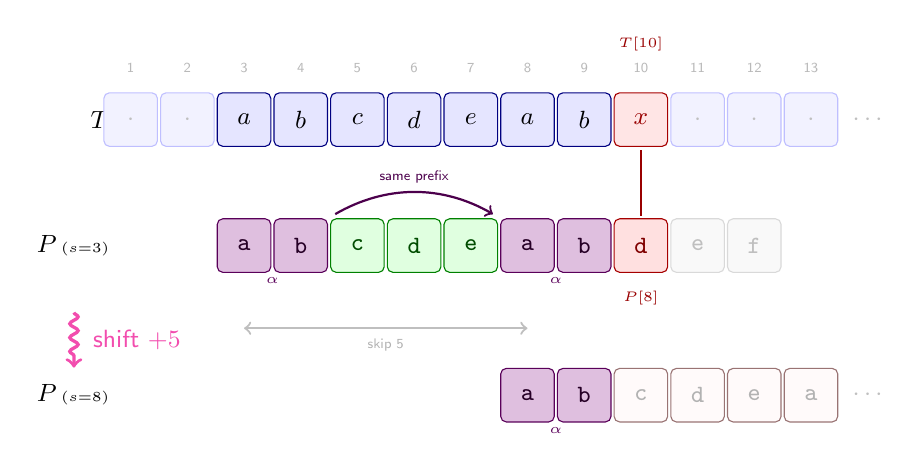
\begin{tikzpicture}[
  cell/.style={
    minimum width=6.8mm, minimum height=6.8mm,
    font=\ttfamily\small, inner sep=0pt,
    text centered, rounded corners=2pt,
  },
  Tdim/.style  ={cell, draw=blue!25,        fill=blue!5,    text=gray!50},
  Tmatch/.style={cell, draw=blue!50!black,  fill=blue!10},
  Txc/.style   ={cell, draw=red!65!black,   fill=red!10,    text=red!60!black},
  Alpha/.style ={cell, draw=violet!70!black,fill=violet!25, text=violet!30!black},
  MC/.style    ={cell, draw=green!50!black, fill=green!12,  text=green!30!black},
  XC/.style    ={cell, draw=red!65!black,   fill=red!12,    text=red!50!black},
  NC/.style    ={cell, draw=gray!30,        fill=gray!5,    text=gray!50},
  AlphaNew/.style={cell, draw=violet!70!black, fill=violet!25, text=violet!30!black},
  NewP/.style  ={cell, draw=pink!60!black,  fill=pink!8,    text=gray!60},
]

\def\cw{0.72}

% ── position indices (1-based) ───────────────────────────
\foreach \i in {1,...,13}
  \node[font=\tiny\sffamily, text=gray!55] at ({(\i-1)*\cw}, 2.85) {\i};

% ── T row ────────────────────────────────────────────────
% T: ··abcdeabx··  (· = unimportant char, 1-based positions)
\node[font=\small\ttfamily, anchor=east] at (-0.15, 2.2) {$T$};
\foreach \i/\c/\sty in {
     1/{\cdot}/Tdim,  2/{\cdot}/Tdim,
     3/a/Tmatch, 4/b/Tmatch, 5/c/Tmatch,
     6/d/Tmatch, 7/e/Tmatch, 8/a/Tmatch, 9/b/Tmatch,
    10/x/Txc,
    11/{\cdot}/Tdim, 12/{\cdot}/Tdim, 13/{\cdot}/Tdim}
  \node[\sty] at ({(\i-1)*\cw}, 2.2) {$\c$};
\node[font=\ttfamily\small, text=gray!50] at (13*\cw, 2.2) {$\cdots$};

% mismatch vertical line
\draw[red!60!black, thick]
  (9*\cw, 0.6+0.38) -- (9*\cw, 2.2-0.38);

% T\kern0pt[10] label above
\node[font=\tiny\sffamily, text=red!60!black, above=2pt]
  at (9*\cw, 2.5+0.38) {$T\kern0pt[10]$};

% ── P at s=3  (y = 0.6) ──────────────────────────────────
% P = a  b  c  d  e  a  b  d  e  f
%     1  2  3  4  5  6  7  8  9  10   (T-positions: 3..12)
\node[font=\small\ttfamily, anchor=east] at (-0.15, 0.6)
  {$P$\,{\tiny$(s{=}3)$}};

% α prefix  P[1..2] → T[3..4]
\node[Alpha] (pa1) at (2*\cw, 0.6) {a};
\node[Alpha] (pa2) at (3*\cw, 0.6) {b};
% middle matched  P[3..5] → T[5..7]
\node[MC] at (4*\cw, 0.6) {c};
\node[MC] at (5*\cw, 0.6) {d};
\node[MC] at (6*\cw, 0.6) {e};
% α suffix  P[6..7] → T[8..9]
\node[Alpha] (pa6) at (7*\cw, 0.6) {a};
\node[Alpha] (pa7) at (8*\cw, 0.6) {b};
% mismatch  P\kern0pt[8] → T\kern0pt[10]
\node[XC]   at (9*\cw, 0.6) {d};
% not compared  P[9..10] → T[11..12]
\node[NC]   at (10*\cw, 0.6) {e};
\node[NC]   at (11*\cw, 0.6) {f};

% P\kern0pt[8] label below mismatch
\node[font=\tiny\sffamily, text=red!60!black, below=2pt]
  at (9*\cw, 0.6-0.38) {$P\kern0pt[8]$};

% α labels
\node[font=\tiny\sffamily, text=violet!70!black, below=8pt]
  at (2.5*\cw, 0.6) {$\alpha$};
\node[font=\tiny\sffamily, text=violet!70!black, below=8pt]
  at (7.5*\cw, 0.6) {$\alpha$};

% curved arrow linking the two α segments
\draw[violet!60!black, thick, ->, bend left=30,
      shorten >=3pt, shorten <=3pt]
  (pa2.north east) to node[above, font=\tiny\sffamily,
                             text=violet!60!black] {same prefix}
  (pa6.north west);

% ── shift annotation ─────────────────────────────────────
\draw[->, magenta!70, very thick, decorate,
      decoration={snake, amplitude=1.5pt, segment length=5pt,
                  post length=4pt}]
  (-1.0*\cw, -0.25) -- (-1.0*\cw, -0.95)
  node[right=3pt, font=\small\sffamily, text=magenta!70,
       pos=0.5] {shift $+5$};

\draw[gray!50, thick, <->]
  (2*\cw, -0.45) -- (7*\cw, -0.45)
  node[midway, below, font=\tiny\sffamily, text=gray!60] {skip 5};

% ── P at s=8  (y = −1.3) ─────────────────────────────────
\node[font=\small\ttfamily, anchor=east] at (-0.15, -1.3)
  {$P$\,{\tiny$(s{=}8)$}};

% α prefix now aligns with the former α suffix
\node[AlphaNew] at (7*\cw, -1.3) {a};
\node[AlphaNew] at (8*\cw, -1.3) {b};
% rest of P
\foreach \i/\c in {9/c, 10/d, 11/e, 12/a}
  \node[NewP] at (\i*\cw, -1.3) {\c};
\node[font=\ttfamily\small, text=gray!50] at (13*\cw, -1.3) {$\cdots$};

% α label
\node[font=\tiny\sffamily, text=violet!70!black, below=8pt]
  at (7.5*\cw, -1.3) {$\alpha$};

\end{tikzpicture}
\caption{%
  KMP shift intuition with $P = \texttt{abcdeabdef}$.
  At shift $s=3$, the algorithm matches $P[1\ldots7] = \texttt{abcdeab}$
  then hits a mismatch at $P\kern0pt[8]$.
  The matched portion ends with $\alpha = \texttt{ab}$, which also appears
  at the very start of $P$ --- so instead of shifting by $1$, we jump
  directly to $s=8$, re-aligning $\alpha$ and resuming from $P\kern0pt[3]$.
}
\label{fig:kmp-shift}
\end{figure}

Basically what the example shows is that if we take the longest prefix\aside{When we say suffix here we mean suffix of the \textbf{matched} portion of $P$, not of $P$ itself. In the example, $\alpha$ is a suffix of $P[1\ldots7]$ but not of the whole $P$.} of $P$ that is also a suffix of the \textbf{matched} portion of $P$, we can shift the pattern so that this prefix is now aligned with the suffix --- and we can resume the search from the character right after this prefix, since we know it must match (otherwise we would have had a mismatch earlier). In other words we have saved some work (namely, five shift indexes) by leveraging the information from the previous comparisons, instead of starting over from scratch, from the very next shift.

But is this correct? Or do we miss some potential matches by jumping directly to $s=8$?

\begin{figure}[H]
  \centering
  
\includegraphics[width=0.38\textwidth]{images/michael-scott.png}
  \caption*{\small ``You miss 100\% of the shots you don't take.'' --- Michael Scott}
\end{figure}

Well, it turns out that this is indeed correct, and we won't miss any matches by doing this. The KMP algorithm is based on this very idea, and it guarantees that we will find all occurrences of $P$ in $T$ without missing any, while also achieving a much better time complexity than the naive approach.

\subsubsection{Preprocessing: computing $sp$ values}
\label{sec:kmp-preprocessing}

To exploit this idea, we need to precompute for every prefix $P[1\ldots i]$ its
\emph{longest proper prefix that is also a suffix}. We write this length as $\spi{i}$\aside{A \emph{proper} prefix/suffix excludes the string itself; $\spi{i}$ is thus an integer.}.

\begin{definition}[$sp$ values]
  Let $P$ be a pattern of length $m$. For each $i \in \{1,\ldots,m\}$, define
  \[
    \spi{i} \;=\; \max\bigl\{\, k < i \mid P[1\ldots k] = P[i-k+1\ldots i] \,\bigr\},
  \]
  i.e.\ the length of the longest proper prefix of $P[1\ldots i]$ that is also a suffix of $P[1\ldots i]$.
\end{definition}

The key observation is that $\spi{i}$ can be computed recursively from $\spi{i-1}$,
giving an efficient $\Oh{m}$ preprocessing algorithm. There are two cases:

\begin{enumerate}
  \item \textbf{Extension is possible.} Let $k = \spi{i-1}$. If $P[k+1] = P\kern0pt[i]$,
        then the longest prefix-suffix of $P[1\ldots i]$ is simply one character longer
        than that of $P[1\ldots i-1]$, so $\spi{i} = k + 1$.

        \textit{Example:} with $P = \texttt{abcdeabdef}$ at $i=7$, we have $\spi{6}=1$
        (the prefix-suffix of $\texttt{abcdea}$ is $\texttt{a}$, length $1$). We check
        $P\kern0pt[2] = \texttt{b}$ against $P\kern0pt[7] = \texttt{b}$: they match, so $\spi{7} = 2$
        (see Figure~\ref{fig:sp-computation}).

  \item \textbf{Extension is not possible.} If $P[k+1] \neq P\kern0pt[i]$, we cannot
        extend the current prefix-suffix. We then ask: what is the longest
        prefix-suffix of the prefix-suffix itself? In other words, we fall back to
        $k \gets \spi{k}$ and try to extend that instead. We repeat this process
        until either a match is found or we reach $k = 0$, in which case $\spi{i} = 0$.

        \textit{Example:} still with $P = \texttt{abcdeabdef}$ at $i=8$, we have
        $\spi{7}=2$ (the prefix-suffix of $\texttt{abcdeab}$ is $\texttt{ab}$). We check
        $P\kern0pt[3] = \texttt{c}$ against $P\kern0pt[8] = \texttt{d}$: no match. We fall back to
        $k \gets \spi{2} = 0$, so we check $P\kern0pt[1] = \texttt{a}$ against $P\kern0pt[8] = \texttt{d}$,
        still no match. We have reached $k = 0$, so $\spi{8} = 0$.
\end{enumerate}

% ── Figure: computing sp\kern0pt[i] from sp[i-1] ─────────────────
\begin{figure}[H]
\centering
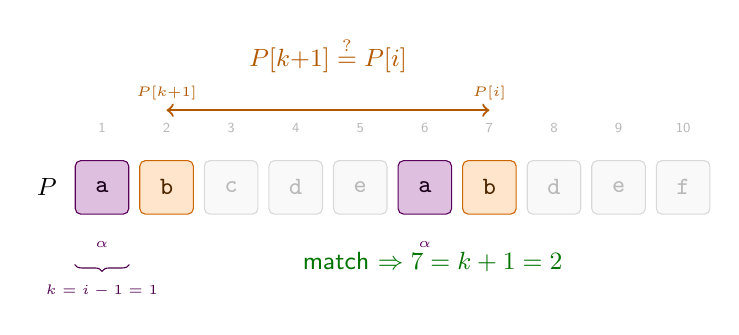
\begin{tikzpicture}[
  cell/.style={
    minimum width=6.8mm, minimum height=6.8mm,
    font=\ttfamily\small, inner sep=0pt,
    text centered, rounded corners=2pt,
  },
  Alpha/.style={cell, draw=violet!70!black, fill=violet!25, text=violet!20!black},
  Cmp/.style  ={cell, draw=orange!80!black, fill=orange!20, text=orange!30!black},
  NC/.style   ={cell, draw=gray!30,         fill=gray!5,    text=gray!55},
]

\def\cw{0.82}

% position indices (1-based)
\foreach \i in {1,...,10}
  \node[font=\tiny\sffamily, text=gray!55] at ({(\i-1)*\cw}, 0.75) {\i};

% P = a  b  c  d  e  a  b  d  e  f
%     1  2  3  4  5  6  7  8  9 10
\node[font=\small\ttfamily, anchor=east] at (-0.45, 0) {$P$};

% P\kern0pt[1] : α prefix (length k = sp_{i-1}(P) = 1)
\node[Alpha] (p1) at (0*\cw, 0) {a};
% P\kern0pt[2] : P[k+1], the comparison character
\node[Cmp]   (p2) at (1*\cw, 0) {b};
% P[3..5] : middle
\node[NC] at (2*\cw, 0) {c};
\node[NC] at (3*\cw, 0) {d};
\node[NC] at (4*\cw, 0) {e};
% P\kern0pt[6] : α suffix of P[1..i-1]  (i-k = 6)
\node[Alpha] (p6) at (5*\cw, 0) {a};
% P\kern0pt[7] : P\kern0pt[i], the current position
\node[Cmp]   (p7) at (6*\cw, 0) {b};
% P[8..10] : not yet processed
\node[NC] at (7*\cw, 0) {d};
\node[NC] at (8*\cw, 0) {e};
\node[NC] at (9*\cw, 0) {f};

% labels above
\node[font=\tiny\sffamily, text=orange!70!black, above=18pt] at (p2.north) {$P[k{+}1]$};
\node[font=\tiny\sffamily, text=orange!70!black, above=18pt] at (p7.north) {$P\kern0pt[i]$};

% α labels below
\node[font=\tiny\sffamily, text=violet!70!black, below=6pt] at (p1.south) {$\alpha$};
\node[font=\tiny\sffamily, text=violet!70!black, below=6pt] at (p6.south) {$\alpha$};

% brace under α prefix
\draw[violet!60!black, decorate,
      decoration={brace, mirror, raise=18pt}]
  (p1.south west) -- (p1.south east)
  node[midway, below=22pt, font=\tiny\sffamily,
       text=violet!60!black] {$k = \spi{i-1} = 1$};

% comparison arrow
\draw[orange!70!black, thick, <->]
  ([yshift=18pt]p2.north) -- ([yshift=18pt]p7.north)
  node[midway, above, font=\small, text=orange!70!black, yshift=10pt]
    {$P[k{+}1] \stackrel{?}{=} P\kern0pt[i]$};

% outcome label
\node[font=\small\sffamily, text=green!45!black, below=20pt]
  at (5*\cw, 0)
  {\checkmark\; match $\Rightarrow \spi{7} = k+1 = 2$};

\end{tikzpicture}
\caption{%
  Computing $\spi{7}$ for $P = \texttt{abcdeabdef}$.
  We know $k = \spi{6} = 1$: the suffix of $P[1\ldots6]$ matching a prefix of $P$
  has length $1$ (namely $\alpha = \texttt{a}$, \textcolor{violet!70!black}{violet}).
  We compare $P[k+1] = P\kern0pt[2] = \texttt{b}$ against $P\kern0pt[i] = P\kern0pt[7] = \texttt{b}$
  (\textcolor{orange!70!black}{orange}): they match, so $\spi{7} = 2$.
}
\label{fig:sp-computation}
\end{figure}

The resulting algorithm is the following:

\begin{algorithm}[H]
  \caption{Computing $sp$ values}
  \KwIn{Pattern $P[1\ldots m]$}
  \KwOut{Array $sp[1\ldots m]$ where $sp\kern0pt[i] = \spi{i}$}
  $sp\kern0pt[1] \gets 0$ \;
  $k \gets 0$ \tcp*{length of current candidate prefix-suffix}
  \For{$i \gets 2$ \KwTo $m$}{
    \While{$k > 0$ \textbf{and} $P[k+1] \neq P\kern0pt[i]$}{
      $k \gets sp\kern0pt[k]$ \tcp*{fall back}
    }
    \If{$P[k+1] = P\kern0pt[i]$}{
      $k \gets k + 1$ \;
    }
    $sp\kern0pt[i] \gets k$ \;
  }
  \Return $sp$
\end{algorithm}

\begin{remark}[{Why fall back to $sp\kern0pt[k]$?}]
  At every point in the loop, $k$ has a precise meaning: it is the length
  of the longest prefix of $P$ that currently matches a suffix of
  $P[1\ldots i{-}1]$.
  In other words,
  \[
    P[1\ldots k] \;=\; P[i-k\ldots i-1],
  \]
  the $k$ characters immediately before position~$i$ are exactly the first $k$
  characters of the pattern.
  When $P[k+1] = P\kern0pt[i]$ we can extend this match by one: $sp\kern0pt[i] = k+1$.
  When $P[k+1] \neq P\kern0pt[i]$ the match of length $k$ cannot be extended, and we
  need a shorter candidate $j < k$ that still satisfies the same property:
  $P[1\ldots j] = P[i-j\ldots i-1]$.

  \smallskip\noindent
  \textbf{Key insight.}
  $P[1\ldots k]$ is not an arbitrary string --- it is a \emph{prefix} of $P$.
  Any valid candidate $j$ must be a prefix of $P$ that also appears as a
  suffix of $P[1\ldots i{-}1]$.
  Two simple observations handle this:
  \begin{itemize}[noitemsep, topsep=2pt]
    \item \emph{Prefix of a prefix is a prefix}: if $P[1\ldots j]$ is a
          prefix of $P[1\ldots k]$, it is a prefix of~$P$.
    \item \emph{Suffix of a suffix is a suffix}: since $P[1\ldots k]$
          is a suffix of $P[1\ldots i{-}1]$ (by the invariant), any suffix of
          $P[1\ldots k]$ of length $j$ is also a suffix of $P[1\ldots i{-}1]$.
  \end{itemize}
  Therefore $j$ is a valid candidate \emph{if and only if} $P[1\ldots j]$ is
  a \emph{border} of $P[1\ldots k]$ (a string that is both a prefix and a
  suffix of it).
  The longest such border is $sp\kern0pt[k]$, already computed during preprocessing.
  Any value strictly between $sp\kern0pt[k]$ and $k$ is, by definition of $sp\kern0pt[k]$,
  not a border of $P[1\ldots k]$ and therefore not a valid candidate --- no
  check is needed.
  We jump directly to $k \gets sp\kern0pt[k]$ and repeat.
  Figure~\ref{fig:sp-fallback-trace} shows this chain for $i=6$, $k=3$.
\end{remark}

\begin{note}[{A fallback that succeeds}]
  Let $P = \texttt{ababcababa}$ and consider $i = 10$.
  We have $k = 4$ since $P[1\ldots 4] = P[6\ldots 9] = \texttt{abab}$.
  Check $P\kern0pt[5] = \texttt{c}$ vs.\ $P\kern0pt[10] = \texttt{a}$: mismatch.
  Could $k'=3$ be a valid candidate?
  It would need $P[1\ldots 3]$ to be a border of $\texttt{abab}$,
  i.e.\ $\texttt{aba} = \texttt{bab}$: no.
  The longest border of $\texttt{abab}$ is $\texttt{ab}$ (length~$2$), so $sp\kern0pt[4]=2$.
  We fall back to $k=2$: $P[1\ldots 2] = P[8\ldots 9] = \texttt{ab}$.
  Check $P\kern0pt[3] = \texttt{a}$ vs.\ $P\kern0pt[10] = \texttt{a}$: \textbf{match}!
  Hence $sp\kern0pt[10] = 3$; skipping $k'=3$ was the only correct move.
\end{note}

\begin{formaldetails}[{Why no candidate between $sp\kern0pt[k]$ and $k$ exists}]
  Suppose for contradiction that $sp\kern0pt[k] < k' < k$ and that $k'$ satisfies
  the same property as $k$, i.e.\ $P[1\ldots k'] = P[i-k'\ldots i-1]$.
  Since $k' < k$, the string $P[i-k'\ldots i-1]$ is a suffix of
  $P[i-k\ldots i-1] = P[1\ldots k]$.
  Combined with $P[1\ldots k']$ being a prefix of $P$, this makes
  $P[1\ldots k']$ a border of $P[1\ldots k]$ of length $k' > sp\kern0pt[k]$,
  contradicting $sp\kern0pt[k]$ being the \emph{longest} proper border of
  $P[1\ldots k]$. \hfill$\square$
\end{formaldetails}

\begin{formaldetails}[Correctness of the $sp$ preprocessing algorithm]
  We prove that at the end of iteration~$i$, $sp\kern0pt[i]$ equals the length of the
  longest proper border of $P[1\ldots i]$.

  \begin{loopproof}
    \item[Precondition]  $P[1\ldots m]$ is given; $sp\kern0pt[1]=0$ and $k=0$ are set before the loop.
    \item[Loop guard]    $i$ ranges from $2$ to $m$.
    \item[Invariant]     At the \emph{start} of iteration~$i$:
                         $k = sp[i{-}1]$, i.e.\ $k$ is the length of the longest
                         proper border of $P[1\ldots i{-}1]$ (and in particular
                         $P[1\ldots k] = P[i{-}k\ldots i{-}1]$).
    \item[Postcondition] $sp\kern0pt[i]$ is correctly set for all $1 \le i \le m$.
  \end{loopproof}

  \lprulesep

  \begin{loopproof}
    \item[Base case]     Before the first iteration ($i=2$), $k=0=sp\kern0pt[1]$
                         since $P[1\ldots 1]$ has no proper border. \checkmark
    \item[Preservation]  Assume the invariant holds at the start of iteration~$i$,
                         i.e.\ $k=sp[i{-}1]$.
                         The inner \textbf{while} loop traverses the border chain
                         $k \to sp\kern0pt[k] \to sp[sp\kern0pt[k]] \to \cdots$, stopping as soon
                         as $P[k{+}1]=P\kern0pt[i]$ or $k=0$.
                         By the border characterisation (a candidate $j$ is valid iff
                         $P[1\ldots j]$ is a border of $P[1\ldots k]$), this finds
                         the longest extendable border.
                         The subsequent \textbf{if} either increments $k$ by one or
                         leaves $k=0$.
                         In both cases $sp\kern0pt[i] \gets k$ is correct, and $k=sp\kern0pt[i]$
                         is the invariant for iteration $i{+}1$. \checkmark
    \item[Postcondition] When the loop exits ($i=m+1$), all $sp\kern0pt[i]$ have been
                         correctly computed. \checkmark
  \end{loopproof}
\end{formaldetails}

\subsubsection*{Step-by-step: Computing $sp$ values}

Let's trace the algorithm on $P = \texttt{ababaca}$.

\begin{enumerate}[noitemsep, topsep=3pt]
  \item \textbf{$i=1$:} By definition $sp\kern0pt[1] = 0$. $k \gets 0$.
  \item \textbf{$i=2$:} $k=0$, $P\kern0pt[1]=\texttt{a} \neq P\kern0pt[2]=\texttt{b}$. $sp\kern0pt[2] = 0$.
  \item \textbf{$i=3$:} $k=0$, $P\kern0pt[1]=\texttt{a} = P\kern0pt[3]=\texttt{a}$. $k \gets k+1 = 1$. $sp\kern0pt[3] = 1$.
  \item \textbf{$i=4$:} $k=1$, $P\kern0pt[2]=\texttt{b} = P\kern0pt[4]=\texttt{b}$. $k \gets k+1 = 2$. $sp\kern0pt[4] = 2$.
  \item \textbf{$i=5$:} $k=2$, $P\kern0pt[3]=\texttt{a} = P\kern0pt[5]=\texttt{a}$. $k \gets k+1 = 3$. $sp\kern0pt[5] = 3$.
  \item \textbf{$i=6$:} $k=3$.
        The invariant gives $P[1\ldots 3] = P[3\ldots 5] = \texttt{aba}$.
        We check $P\kern0pt[4]=\texttt{b}$ against $P\kern0pt[6]=\texttt{c}$: mismatch, so we fall back.
        The fallback chain is shown in Figure~\ref{fig:sp-fallback-trace}:
        \begin{itemize}[noitemsep, topsep=2pt]
          \item $k \gets sp\kern0pt[3] = 1$: the longest border of $\texttt{aba}$ is $\texttt{a}$
                (length~$1$). Check $P\kern0pt[2]=\texttt{b}$ against $P\kern0pt[6]=\texttt{c}$: mismatch.
          \item $k \gets sp\kern0pt[1] = 0$: the longest border of $\texttt{a}$ is empty.
                Check $P\kern0pt[1]=\texttt{a}$ against $P\kern0pt[6]=\texttt{c}$: mismatch.
          \item $k=0$: no candidate left. $sp\kern0pt[6] = 0$.
        \end{itemize}

% ── Figure: sp-fallback-trace ─────────────────────────────
\begin{figure}[H]
\centering
\begin{tikzpicture}[
  cell/.style={
    minimum width=6.5mm, minimum height=6.5mm,
    font=\ttfamily\small, inner sep=0pt,
    text centered, rounded corners=2pt,
  },
  Alpha/.style={cell, draw=violet!70!black, fill=violet!25, text=violet!20!black},
  Try/.style  ={cell, draw=orange!75!black, fill=orange!12, text=orange!60!black},
  NC/.style   ={cell, draw=gray!30,         fill=gray!5,    text=gray!55},
  Cur/.style  ={cell, draw=red!60!black,    fill=red!8,     text=red!55!black},
  Pointer/.style={-Stealth, thick, red!65!black},
]
\def\cw{0.82}

% ── indices ──────────────────────────────────────────────────────────
\foreach \i in {1,...,7}
  \node[font=\tiny\sffamily, text=gray!55] at ({(\i-1)*\cw}, 2.2) {\i};

% ── full P reference row ─────────────────────────────────────────────
\node[font=\small\ttfamily, anchor=east] at (-0.55, 1.4) {$P$};
\foreach \i/\c in {1/a, 2/b, 3/a, 4/b, 5/a, 7/a}
  \node[NC] at ({(\i-1)*\cw}, 1.4) {\c};
\node[Cur] (pi) at (5*\cw, 1.4) {c};
\node[font=\tiny\sffamily, text=red!60!black, below=3pt] at (pi.south) {$P\kern0pt[6]=P\kern0pt[i]$};

% ── header ───────────────────────────────────────────────────────────
\node[font=\tiny\itshape, text=gray!60, anchor=west] at (0, 0.45)
  {All borders of $P[1..5]=\texttt{ababa}$, tried longest first:};

% ══ candidate 1: k = 3  (border "aba", length 3) ═════════════════════
\node[font=\tiny\sffamily, text=gray!60, anchor=east] at (-0.1*\cw, -0.7) {$k{=}3$};

\node[Alpha] (s1c3) at (2*\cw, -0.7) {a};
\node[Alpha] (s1c4) at (3*\cw, -0.7) {b};
\node[Alpha] (s1c5) at (4*\cw, -0.7) {a};
\node[Try]   (s1x)  at (5*\cw, -0.7) {b};   % P[k+1]=P\kern0pt[4]

\node[font=\tiny\sffamily, text=red!65!black, right=5pt] at (s1x.east)
  {$P[k{+}1]{=}P\kern0pt[4]{=}\texttt{b}\ \neq\ \texttt{c}{=}P\kern0pt[i]$};

\draw[decorate, decoration={brace, mirror, raise=8pt}, violet!65!black]
  (s1c3.south west) -- (s1c5.south east)
  node[midway, below=12pt, font=\tiny\sffamily, text=violet!60!black]
    {$P[3..5] = P[1..3]$};

\draw[Pointer] (3*\cw, -1.9) -- (0, -1.9)
  node[midway, below=2pt, font=\tiny\sffamily, text=red!65!black]
    {$k \gets sp\kern0pt[3]=1$ \enspace(longest border of $\texttt{aba}$ is $\texttt{a}$)};

% ══ candidate 2: k = 1  (border "a", length 1) ═══════════════════════
\node[font=\tiny\sffamily, text=gray!60, anchor=east] at (-0.1*\cw, -2.8) {$k{=}1$};

\node[Alpha] (s2c5) at (4*\cw, -2.8) {a};
\node[Try]   (s2x)  at (5*\cw, -2.8) {b};   % P[k+1]=P\kern0pt[2]

\node[font=\tiny\sffamily, text=red!65!black, right=5pt] at (s2x.east)
  {$P[k{+}1]{=}P\kern0pt[2]{=}\texttt{b}\ \neq\ \texttt{c}{=}P\kern0pt[i]$};

\draw[decorate, decoration={brace, mirror, raise=8pt}, violet!65!black]
  (s2c5.south west) -- (s2c5.south east)
  node[midway, below=12pt, font=\tiny\sffamily, text=violet!60!black]
    {$P[5..5] = P[1..1]$};

\draw[Pointer] (1*\cw, -3.9) -- (0, -3.9)
  node[midway, below=2pt, font=\tiny\sffamily, text=red!65!black]
    {$k \gets sp\kern0pt[1]=0$ \enspace(border of $\texttt{a}$ is empty)};

% ══ candidate 3: k = 0  (empty border) ═══════════════════════════════
\node[font=\tiny\sffamily, text=gray!60, anchor=east] at (-0.1*\cw, -4.9) {$k{=}0$};

\node[Try] (s3x) at (0*\cw, -4.9) {a};   % P[k+1]=P\kern0pt[1]

\node[font=\tiny\sffamily, text=red!65!black, right=5pt] at (s3x.east)
  {$P[k{+}1]{=}P\kern0pt[1]{=}\texttt{a}\ \neq\ \texttt{c}{=}P\kern0pt[i]$
   \enspace$\Rightarrow$\enspace $sp\kern0pt[6]=0$};

\end{tikzpicture}
\caption{Fallback chain at step $i=6$ for $P=\texttt{ababaca}$.
  The three rows show \emph{all} borders of $P[1..5]=\texttt{ababa}$
  (lengths $3$, $1$, $0$), tried longest first.
  For each candidate $k$, the violet cells show the matched suffix
  $P[i-k..i-1]=P[1..k]$; the orange cell is the character $P[k+1]$
  we would need at position $i$ to extend it.
  All three fail, so $sp\kern0pt[6]=0$.}
\label{fig:sp-fallback-trace}
\end{figure}

  \item \textbf{$i=7$:} $k=0$, $P\kern0pt[1]=\texttt{a} = P\kern0pt[7]=\texttt{a}$. $k \gets k+1 = 1$. $sp\kern0pt[7] = 1$.
\end{enumerate}

\begin{center}
\begin{tabular}{rccccccc}
  \toprule
  $i$    & 1 & 2 & 3 & 4 & 5 & 6 & 7 \\
  \midrule
  $P\kern0pt[i]$ & \texttt{a} & \texttt{b} & \texttt{a} & \texttt{b} & \texttt{a} & \texttt{c} & \texttt{a} \\
  $sp\kern0pt[i]$ & 0 & 0 & 1 & 2 & 3 & 0 & 1 \\
  \bottomrule
\end{tabular}
\end{center}

\begin{remark}
  The ``fall back to the $sp$ value of the current $sp$ value'' is the recursive
  heart of KMP: the same shift logic used during the search phase is also used
  during preprocessing.
\end{remark}

\begin{exercise}
  Design an algorithm that, given a pattern $P$ of length $m$, computes
  $\spi{i}$ for every $i \in \{1, \ldots, m\}$ in $\Oh{m}$ time.

  \medskip
  \textit{Hints:}
  \begin{enumerate}
    \item Try to express $\spi{i}$ in terms of $\spi{i-1}$.
          What is the relationship between the longest prefix-suffix of
          $P[1\ldots i]$ and that of $P[1\ldots i-1]$?
    \item There are two cases depending on whether $P[\spi{i-1}+1]$ equals
          $P\kern0pt[i]$ or not. What can you do in each case?
    \item For the harder case, think recursively: if you cannot extend
          a prefix-suffix of length $k$, which shorter candidate should
          you try next?
  \end{enumerate}
\end{exercise}

\begin{exercise}[Period of a string]
  The \emph{period} of a string $S$ of length $n$ is the smallest integer $p \geq 1$
  such that $S[i] = S[i+p]$ for all $1 \leq i \leq n - p$.
  Equivalently, $p$ is the length of the shortest string $\Pi$ such that $S$ is a
  prefix of $\Pi^{\infty} = \Pi\Pi\Pi\cdots$

  Design an $\Oh{n}$-time algorithm that, given $S$, computes its period.

  \medskip
  \textit{Hints:}
  \begin{enumerate}
    \item Compute the $sp$ values of $S$.
    \item What is the relationship between $sp_n(S)$ and the period of $S$?
          In particular, is $n - sp_n(S)$ always a period?
    \item Is it always the \emph{shortest} period?  What additional condition on
          $sp_n(S)$ guarantees minimality?
  \end{enumerate}
\end{exercise}

\begin{intermezzo}{Amortised analysis — the credit method}

Some algorithms contain operations that look expensive in isolation but are cheap
\emph{on average} over any sequence of calls.
\emph{Amortised analysis} makes this precise by distributing the cost of occasional
expensive operations across the many cheap ones that made them possible.

A clean way to formalise this is the \textbf{credit method}.

\begin{definition}[Credit method]
  Assign each operation an \emph{amortised cost} $\hat{c}$ (which we choose freely).
  When an operation with real cost $c$ runs:
  \begin{itemize}[nosep]
    \item if $\hat{c} > c$, the surplus $\hat{c} - c$ is deposited as \emph{credits} into a bank;
    \item if $\hat{c} < c$, the deficit $c - \hat{c}$ is withdrawn from the bank.
  \end{itemize}
  \textbf{Invariant:} the bank balance must never go negative.

  \medskip
  \textbf{Consequence:} since the bank starts at $0$ and never goes below $0$,
  \[
    \sum_{i} c_i \;\leq\; \sum_{i} \hat{c}_i,
  \]
  i.e.\ the total real cost is bounded by the total amortised cost.
\end{definition}

\paragraph{Example: stack with \textsc{push} and \textsc{multi-pop}.}
Consider a stack supporting two operations:
\begin{itemize}[nosep]
  \item $\textsc{push}(x)$: push element $x$ onto the stack; real cost $1$.
  \item $\textsc{multi-pop}(k)$: pop the top $\min(k,\,|S|)$ elements; real cost $=$ number of elements actually popped.
\end{itemize}
A single \textsc{multi-pop} can cost $\Th{n}$, so a naive worst-case analysis gives
$\Oh{n^2}$ for $n$ operations.  Amortised analysis does much better.

\medskip
\textbf{Credit assignment.}
Attach $1$ credit to each element at the moment it is pushed:
\begin{itemize}[nosep]
  \item $\textsc{push}$: amortised cost $\hat{c} = 2$
        (pay $1$ for the real push, deposit $1$ credit \emph{on the element}).
  \item $\textsc{multi-pop}(k)$: amortised cost $\hat{c} = 0$
        (use the $1$ credit stored on each popped element to pay for its removal).
\end{itemize}
The bank balance equals the number of elements on the stack, which is always $\geq 0$,
so the invariant holds.

\begin{example}[Credit trace for a stack]
  The table below traces the sequence
  \textsc{push}(a), \textsc{push}(b), \textsc{push}(c), \textsc{multi-pop}(2),
  \textsc{push}(d), \textsc{push}(e), \textsc{multi-pop}(3).

  \medskip
  \begin{center}
  \begin{tabular}{lcccc}
    \toprule
    Operation              & Stack after  & Real cost & Amortised cost & Bank \\
    \midrule
    \textsc{push}(a)       & $[a]$        & 1         & 2              & 1    \\
    \textsc{push}(b)       & $[a,b]$      & 1         & 2              & 2    \\
    \textsc{push}(c)       & $[a,b,c]$    & 1         & 2              & 3    \\
    \textsc{multi-pop}(2)  & $[a]$        & 2         & 0              & 1    \\
    \textsc{push}(d)       & $[a,d]$      & 1         & 2              & 2    \\
    \textsc{push}(e)       & $[a,d,e]$    & 1         & 2              & 3    \\
    \textsc{multi-pop}(3)  & $[\,]$       & 3         & 0              & 0    \\
    \midrule
    \textbf{Total}         &              & \textbf{10} & \textbf{10}  &      \\
    \bottomrule
  \end{tabular}
  \end{center}

  \medskip
  The bank never goes negative, confirming the invariant.
  The total real cost $10$ is indeed $\leq$ the total amortised cost $10$.
\end{example}

\begin{lemma}
  Any sequence of $n$ \textsc{push} and \textsc{multi-pop} operations on an initially
  empty stack costs $\Oh{n}$ in total.
\end{lemma}
\begin{proof}
  There are at most $n$ pushes, each with amortised cost $2$, and all \textsc{multi-pop}s
  have amortised cost $0$.  The total amortised cost is therefore at most $2n$.
  By the credit-method bound, the total real cost is at most $2n = \Oh{n}$.
\end{proof}

\end{intermezzo}

\subsubsection{Application to KMP preprocessing}

The $sp$-computation algorithm runs in $\Oh{m}$ total time despite the nested loops.
We apply the credit method with $k$ as the potential: credits measure how much $k$
can still decrease.

\begin{itemize}[nosep]
  \item $k$ increases by at most $1$ per outer iteration (there are $m-1$ iterations,
        so $k$ grows at most $m-1$ times in total).
  \item Each execution of the inner \textbf{while} body sets $k \gets sp\kern0pt[k] < k$,
        strictly decreasing $k$.
  \item $k \geq 0$ always holds.
\end{itemize}

Assign amortised cost $2$ to each outer step that increments $k$ (real cost $1$ plus
deposit $1$ credit), and amortised cost $0$ to each inner iteration that decrements $k$
(use the saved credit).  The bank balance equals $k \geq 0$, so the invariant holds,
and the total number of inner iterations is at most the total number of increments,
which is $\Oh{m}$.
Together with the $\Oh{m}$ overhead of the outer loop, the total preprocessing time is $\Oh{m}$.

\begin{example}
  Consider the pattern $P = \texttt{aaaaa}$ of length $5$. The $sp$ values are
  $sp\kern0pt[1] = 0$, $sp\kern0pt[2] = 1$, $sp\kern0pt[3] = 2$, $sp\kern0pt[4] = 3$, $sp\kern0pt[5] = 4$.
  The variable $k$ starts at $0$ and increases to $1$, then to $2$, then to $3$, then to $4$,
  as we process each character of $P$. There are no decreases in this case, so the inner loop
  runs only once per outer iteration, for a total of $\Oh{m}$ time.
\end{example}

\subsubsection{The search phase}

Once the $sp$ array is computed, we scan $T$ left-to-right, maintaining $j$: the number of
characters of $P$ currently matched.

\begin{algorithm}[H]
  \caption{KMP search}
  \KwIn{Text $T[1\ldots n]$, pattern $P[1\ldots m]$, precomputed $sp[1\ldots m]$}
  \KwOut{All starting positions $s$ where $P$ occurs in $T$}
  $j \gets 0$ \tcp*{characters of $P$ matched so far}
  \For{$i \gets 1$ \KwTo $n$}{
    \While{$j > 0$ \textbf{and} $P[j+1] \neq T\kern0pt[i]$}{
      $j \gets sp\kern0pt[j]$ \tcp*{fall back along the border chain}
    }
    \If{$P[j+1] = T\kern0pt[i]$}{
      $j \gets j + 1$ \;
    }
    \If{$j = m$}{
      \textbf{output} $i - m + 1$ \tcp*{occurrence starting here}
      $j \gets sp\kern0pt[j]$ \tcp*{continue searching}
    }
  }
\end{algorithm}

Figure~\ref{fig:kmp-search-trace} traces the search on a concrete example,
showing how $sp$ values let the algorithm carry previously matched characters
across fallbacks instead of starting from scratch.

% ── Figure: KMP search trace ──────────────────────────────
\begin{figure}[H]
\centering
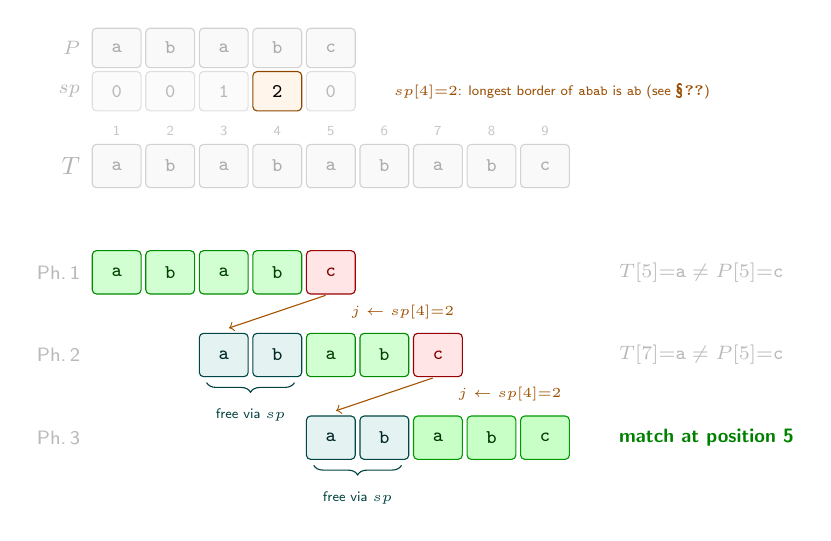
\begin{tikzpicture}[
  cell/.style={
    minimum width=6.2mm, minimum height=5.5mm,
    font=\ttfamily\scriptsize, inner sep=0pt,
    text centered, rounded corners=1.5pt,
  },
  T/.style    ={cell, draw=gray!35,         fill=gray!5,    text=gray!65},
  Carry/.style={cell, draw=teal!55!black,   fill=teal!10,   text=teal!30!black},
  New/.style  ={cell, draw=green!55!black,  fill=green!18,  text=green!25!black},
  Fail/.style ={cell, draw=red!60!black,    fill=red!10,    text=red!50!black},
  Win/.style  ={cell, draw=green!60!black,  fill=green!22,  text=green!20!black},
  SP/.style   ={cell, draw=gray!25,         fill=gray!3,    text=gray!55},
  SPhi/.style ={cell, draw=orange!55!black, fill=orange!8,  text=black},
]
\def\cw{0.68}

% ── sp array for P = ababc ────────────────────────────────
\node[font=\scriptsize\sffamily, text=gray!55, anchor=east]
  at ({-0.5*\cw}, 1.50) {$P$};
\foreach \j/\c in {1/a,2/b,3/a,4/b,5/c}
  \node[T, minimum height=5mm] at ({(\j-1)*\cw}, 1.50) {\c};

\node[font=\scriptsize\sffamily, text=gray!55, anchor=east]
  at ({-0.5*\cw}, 0.95) {$sp$};
\node[SP,   minimum height=5mm] at ({0*\cw}, 0.95) {0};
\node[SP,   minimum height=5mm] at ({1*\cw}, 0.95) {0};
\node[SP,   minimum height=5mm] at ({2*\cw}, 0.95) {1};
\node[SPhi, minimum height=5mm] at ({3*\cw}, 0.95) {2};   % sp\kern0pt[4]=2, key value
\node[SP,   minimum height=5mm] at ({4*\cw}, 0.95) {0};
\node[font=\tiny\sffamily, text=orange!60!black, anchor=west]
  at ({5.0*\cw}, 0.95) {$sp\kern0pt[4]{=}2$: longest border of \texttt{abab} is \texttt{ab}
  (see \S\ref{sec:kmp-preprocessing})};

% ── T row ─────────────────────────────────────────────────
\foreach \j in {1,...,9}
  \node[font=\tiny\sffamily, text=gray!45] at ({(\j-1)*\cw}, 0.45) {\j};
\node[font=\small\sffamily, text=gray!60, anchor=east] at ({-0.5*\cw},0){$T$};
\foreach \j/\c in {1/a,2/b,3/a,4/b,5/a,6/b,7/a,8/b,9/c}
  \node[T] at ({(\j-1)*\cw},0){\c};

% ── Phase 1: offset=0, 4 new matches, fail at T\kern0pt[5] ────────
\node[font=\scriptsize\sffamily, text=gray!55, anchor=east]
  at ({-0.5*\cw},{-1.35}){Ph.\,1};
\foreach \j/\c in {1/a,2/b,3/a,4/b}
  \node[New]  at ({(\j-1)*\cw},{-1.35}){\c};
\node[Fail] at ({4*\cw},{-1.35}){c};
\node[font=\scriptsize\sffamily, text=gray!55, anchor=west]
  at ({9.2*\cw},{-1.35}){$T\kern0pt[5]{=}\texttt{a}\neq P\kern0pt[5]{=}\texttt{c}$};

% fallback arrow Phase 1 → Phase 2
\draw[->, orange!65!black, shorten >=2pt, shorten <=2pt]
  ({4*\cw},{-1.62}) -- ({2*\cw},{-2.08});
\node[font=\tiny\sffamily, text=orange!62!black, anchor=west]
  at ({4.2*\cw},{-1.85}){$j\gets sp\kern0pt[4]{=}2$};

% ── Phase 2: offset=2, 2 carry + 2 new, fail at T\kern0pt[7] ──────
\node[font=\scriptsize\sffamily, text=gray!55, anchor=east]
  at ({-0.5*\cw},{-2.40}){Ph.\,2};
\node[Carry] at ({2*\cw},{-2.40}){a};
\node[Carry] at ({3*\cw},{-2.40}){b};
\node[New]   at ({4*\cw},{-2.40}){a};
\node[New]   at ({5*\cw},{-2.40}){b};
\node[Fail]  at ({6*\cw},{-2.40}){c};
% carry brace
\draw[teal!50!black, decorate,
      decoration={brace, mirror, amplitude=3.5pt, raise=2pt}]
  ({1.68*\cw},{-2.68}) -- ({3.32*\cw},{-2.68})
  node[midway, below=8pt, font=\tiny\sffamily, text=teal!50!black]
    {free via $sp$};
\node[font=\scriptsize\sffamily, text=gray!55, anchor=west]
  at ({9.2*\cw},{-2.40}){$T\kern0pt[7]{=}\texttt{a}\neq P\kern0pt[5]{=}\texttt{c}$};

% fallback arrow Phase 2 → Phase 3
\draw[->, orange!65!black, shorten >=2pt, shorten <=2pt]
  ({6*\cw},{-2.67}) -- ({4*\cw},{-3.13});
\node[font=\tiny\sffamily, text=orange!62!black, anchor=west]
  at ({6.2*\cw},{-2.90}){$j\gets sp\kern0pt[4]{=}2$};

% ── Phase 3: offset=4, 2 carry + 3 new = MATCH ────────────
\node[font=\scriptsize\sffamily, text=gray!55, anchor=east]
  at ({-0.5*\cw},{-3.45}){Ph.\,3};
\node[Carry] at ({4*\cw},{-3.45}){a};
\node[Carry] at ({5*\cw},{-3.45}){b};
\node[Win]   at ({6*\cw},{-3.45}){a};
\node[Win]   at ({7*\cw},{-3.45}){b};
\node[Win]   at ({8*\cw},{-3.45}){c};
% carry brace
\draw[teal!50!black, decorate,
      decoration={brace, mirror, amplitude=3.5pt, raise=2pt}]
  ({3.68*\cw},{-3.73}) -- ({5.32*\cw},{-3.73})
  node[midway, below=8pt, font=\tiny\sffamily, text=teal!50!black]
    {free via $sp$};
\node[font=\scriptsize\bfseries\sffamily, text=green!50!black, anchor=west]
  at ({9.2*\cw},{-3.45}){match at position~5};

\end{tikzpicture}
\caption{%
  KMP search for $P{=}\texttt{ababc}$ ($m{=}5$) in $T{=}\texttt{ababababc}$ ($n{=}9$).
  The $sp$ array for $P$ is shown at the top
  (cf.\ the preprocessing in \S\ref{sec:kmp-preprocessing}).
  \textcolor{green!55!black}{Green}: characters newly matched in this phase.
  \textcolor{teal!55!black}{Teal}: characters carried for free from the previous
  phase via $j\gets sp\kern0pt[j]$.
  \textcolor{red!55!black}{Red}: mismatch.
  After each fallback, the algorithm reuses the last $sp\kern0pt[j]$ matched characters
  without any comparison, then continues from where it left off in $T$.
}
\label{fig:kmp-search-trace}
\end{figure}

The same amortised argument applies: $j$ increases by at most $1$ per outer step and each
inner fallback strictly decreases $j \geq 0$, so the inner loop runs $\Oh{n}$ times in total.

\begin{theorem}
  The KMP algorithm finds all occurrences of $P$ in $T$ in $\Oh{n + m}$ time.
\end{theorem}

% ══════════════════════════════════════════════════════════════════
\subsection{Z-Algorithm}
% ══════════════════════════════════════════════════════════════════

\subsubsection{Definition}

The Z-algorithm is a second linear-time preprocessing approach.
Where $\spi{i}$ looks \emph{backward} (longest prefix that is also a suffix of $P[1\ldots i]$),
the Z-value $Z_i$ looks \emph{forward} from position $i$.

\begin{definition}[Z values]
  Let $A$ be a string of length $n$. For $i \geq 2$, define
  \[
    Z_i(A) \;=\;
    \begin{cases}
      0 & \text{if } A[i] \neq A[1],\\[2pt]
      \max\bigl\{\, \ell > 0 \mid A[1,\ell] = A[i,\,i+\ell-1] \,\bigr\} & \text{otherwise.}
    \end{cases}
  \]
  In words, $Z_i(A)$ is the length of the longest prefix of $A$ that matches $A$ starting
  at position $i$, as shown in Figure~\ref{fig:z-values-example}.
\end{definition}

% ── Figure: Z-values example ──────────────────────────────
\begin{figure}[H]
\centering
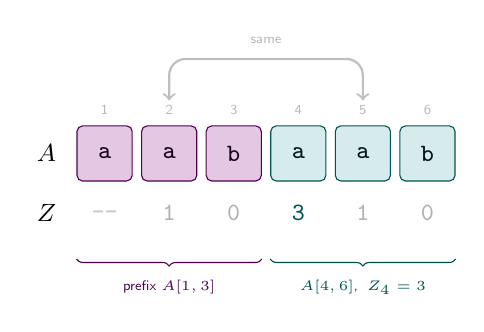
\begin{tikzpicture}[
  cell/.style={
    minimum width=7mm, minimum height=7mm,
    font=\ttfamily\small, inner sep=0pt,
    text centered, rounded corners=2pt,
  },
  Pfx/.style={cell, draw=violet!65!black, fill=violet!22, text=violet!20!black},
  Occ/.style={cell, draw=teal!65!black,   fill=teal!16,   text=teal!20!black},
  NC/.style ={cell, draw=gray!35,         fill=gray!6,    text=gray!55},
]
\def\cw{0.82}

% position indices
\foreach \i in {1,...,6}
  \node[font=\tiny\sffamily, text=gray!55] at ({(\i-1)*\cw}, 1.45) {\i};

% string row: A = a a b a a b
\node[font=\small\ttfamily, anchor=east] at (-0.6*\cw, 0.9) {$A$};
\node[Pfx] (c1) at (0*\cw, 0.9) {a};
\node[Pfx] (c2) at (1*\cw, 0.9) {a};
\node[Pfx] (c3) at (2*\cw, 0.9) {b};
\node[Occ] (c4) at (3*\cw, 0.9) {a};
\node[Occ] (c5) at (4*\cw, 0.9) {a};
\node[Occ] (c6) at (5*\cw, 0.9) {b};

% Z-values row - moved up
\node[font=\small\sffamily, anchor=east] at (-0.6*\cw, 0.15) {$Z$};
\node[font=\small\ttfamily, text=gray!45]                at (0*\cw, 0.15) {--};
\node[font=\small\ttfamily, text=gray!60]                at (1*\cw, 0.15) {1};
\node[font=\small\ttfamily, text=gray!60]                at (2*\cw, 0.15) {0};
\node[font=\small\bfseries\ttfamily, text=teal!70!black] at (3*\cw, 0.15) {3};
\node[font=\small\ttfamily, text=gray!60]                at (4*\cw, 0.15) {1};
\node[font=\small\ttfamily, text=gray!60]                at (5*\cw, 0.15) {0};

% braces showing the two matching blocks - moved down to clear Z row
\draw[violet!60!black, decorate, decoration={brace, mirror, raise=28pt}]
  (c1.south west) -- (c3.south east)
  node[midway, below=32pt, font=\tiny\sffamily, text=violet!65!black]
    {prefix $A[1,3]$};
\draw[teal!60!black, decorate, decoration={brace, mirror, raise=28pt}]
  (c4.south west) -- (c6.south east)
  node[midway, below=32pt, font=\tiny\sffamily, text=teal!65!black]
    {$A[4,6]$,\; $Z_4=3$};

% curved arrow above showing the two blocks are equal - slightly lowered
\draw[gray!50, thick, <->, rounded corners=6pt, shorten >=2pt, shorten <=2pt]
  ([yshift=7pt]c2.north) -- ([yshift=24pt]c2.north) --
  node[above=2pt, font=\tiny\sffamily, text=gray!55] {same}
  ([yshift=24pt]c5.north) -- ([yshift=7pt]c5.north);

\end{tikzpicture}
\caption{%
  Z values for $A = \texttt{aabaab}$ ($n=6$).
  The prefix $A[1,3] = \texttt{aab}$ (\textcolor{violet!65!black}{violet})
  reappears at position $4$ (\textcolor{teal!65!black}{teal}), giving $Z_4 = 3$.
  Also $Z_2 = Z_5 = 1$ since $A[1]=A[2]=A[5]=\texttt{a}$, and
  $Z_3=Z_6=0$ since $A[3]=A[6]=\texttt{b}\neq A[1]$.
  $Z_1$ is left undefined.
}
\label{fig:z-values-example}
\end{figure}

\paragraph{Connection to pattern matching.}
Choose a separator $\$\notin\Sigma$ and form $A = P\$T$ (of length $m+1+n$).
For any index $i$ in the $T$-part of $A$ (i.e.\ $i > m+1$):
\[
  Z_i(P\$T) = m
  \quad\iff\quad
  P \text{ occurs in } T \text{ starting at position } i - m - 1.
\]
The separator prevents $Z_i$ from exceeding $m$, so equality with $m$ detects all occurrences.

\begin{formaldetails}[{Proof of the connection}]
  Write $A = P\$T$ and fix $i > m+1$ (i.e.\ $i$ is in the $T$-part of $A$).

  \smallskip
  \textbf{The separator bounds $Z_i \leq m$.}
  If $Z_i > m$ then $A[i\ldots i+m] = A[1\ldots m+1]$, so in particular
  $A[i+m] = A[m+1] = \$$.
  But $i+m > 2m+1 > m+1$, so $A[i+m]$ lies in the $T$-part of $A$, hence
  $A[i+m] \in \Sigma$.
  Since $\$ \notin \Sigma$ we have a contradiction: $Z_i \leq m$.

  \smallskip
  \textbf{($\Rightarrow$)}
  Suppose $Z_i = m$.
  Then $A[i\ldots i+m-1] = A[1\ldots m] = P$.
  Since $A[i+j-1] = T[i-m-1+j-1]$ for $j = 1,\ldots,m$, this gives
  $T[i-m-1\ldots i-1] = P$, i.e.\ $P$ occurs at position $i-m-1$ in $T$.

  \smallskip
  \textbf{($\Leftarrow$)}
  Suppose $P$ occurs at position $j = i - m - 1$ in $T$, i.e.\
  $T[j\ldots j+m-1] = P$.
  Then $A[i\ldots i+m-1] = T[j\ldots j+m-1] = P = A[1\ldots m]$,
  so $Z_i \geq m$.
  Combined with $Z_i \leq m$ we get $Z_i = m$. \hfill$\square$
\end{formaldetails}

\begin{example}
  Let $P = \texttt{aba}$ ($m=3$) and $T = \texttt{ababac}$ ($n=6$).
  Form $A = \texttt{aba\$ababac}$ and compute $Z$ values for positions $i > 4$:

  \[
    \begin{array}{c|cccccccccc}
      i     & 1 & 2 & 3 & 4 & 5 & 6 & 7 & 8 & 9 & 10 \\
      A[i]  & \texttt{a} & \texttt{b} & \texttt{a} & \texttt{\$}
            & \texttt{a} & \texttt{b} & \texttt{a} & \texttt{b} & \texttt{a} & \texttt{c} \\
      Z_i   & - & 0 & 1 & 0 & \mathbf{3} & 0 & \mathbf{3} & 0 & 1 & 0
    \end{array}
  \]

  The two positions with $Z_i = 3 = m$ are $i = 5$ and $i = 7$, corresponding
  to occurrences of $P$ in $T$ starting at positions $5-3-1=1$ and $7-3-1=3$.
  Indeed $T[1\ldots 3] = \texttt{aba}$ and $T[3\ldots 5] = \texttt{aba}$. \checkmark
\end{example}

\subsubsection{Computing Z values: the Z-box algorithm}

A naive computation of all Z values costs $\Oh{n^2}$: for each $i$, compare
character by character until a mismatch.

\paragraph{Intuition: reuse past work.}
Suppose we have processed positions $2, \ldots, i{-}1$ and at some earlier
position $l$ we found $Z_l = z$, i.e.\ $A[l\ldots l{+}z{-}1] = A[1\ldots z]$.
Call the interval
\[
  [l,\; r], \quad r = l + z - 1
\]
a \emph{Z-box}: a contiguous block that we \emph{know} is an exact copy of the
prefix $A[1\ldots z]$.

Now suppose we want $Z_i$ and $i$ falls \emph{inside} the box ($l \le i \le r$).
Let $k = i{-}l{+}1$ be the \emph{mirror} position of $i$ in the prefix.  Since
the box says $A[l\ldots r] = A[1\ldots r{-}l{+}1]$, we immediately know
\[
  A[i] = A[k],\quad A[i{+}1] = A[k{+}1],\quad \ldots,\quad A[r] = A[r{-}l{+}1].
\]
Whatever is already recorded in $Z_k$ — the length of the match starting at
$k$ in the prefix — is available at $i$ \emph{for free}, without any character
comparisons.  The only open question is whether the match at $i$ extends beyond
$r$, which requires at most one fresh comparison per step.

\paragraph{The Z-box invariant.}
The algorithm maintains the Z-box $[l, r]$ with the \textbf{largest right endpoint}
seen so far:
\[
  r = l + Z_l(A) - 1 \quad (\text{maximised over all processed positions}).
\]
Figure~\ref{fig:z-abstract} shows this setup schematically.

% ── Figure: Z-box abstract schematic ─────────────────────
\begin{figure}[H]
\centering
\resizebox{\linewidth}{!}{%
\begin{tikzpicture}[
  cell/.style={
    minimum width=7.5mm, minimum height=6.5mm,
    inner sep=0pt, text centered, rounded corners=1.5pt,
  },
  NC/.style  ={cell, draw=gray!30,         fill=gray!5},
  Pfx/.style ={cell, draw=violet!55!black, fill=violet!12},
  PfxK/.style={cell, draw=orange!75!black, fill=violet!12, line width=0.9pt},
  Box/.style ={cell, draw=teal!60!black,   fill=teal!12},
  BoxI/.style={cell, draw=orange!75!black, fill=teal!12,   line width=0.9pt},
  Grn/.style ={cell, draw=green!55!black,  fill=green!18},
  Fail/.style={cell, draw=red!60!black,    fill=red!10},
]
\def\cw{0.80}

% ── Position index header ─────────────────────────────────
\foreach \j in {1,...,12}
  \node[font=\tiny\sffamily, text=gray!45] at ({(\j-1)*\cw}, 0.85) {\j};

% ── SCHEMATIC ROW: general Z-box setup ───────────────────
\node[font=\small\sffamily, text=gray!55, anchor=east] at ({-0.5*\cw},0){$A$};
\node[Pfx]  at ({0*\cw},0){}; \node[Pfx]  at ({1*\cw},0){};
\node[PfxK] at ({2*\cw},0){}; % k=3
\node[Pfx]  at ({3*\cw},0){}; \node[Pfx]  at ({4*\cw},0){}; % Z_l=5
\node[NC]   at ({5*\cw},0){}; % gap
\node[Box]  at ({6*\cw},0){}; % l=7
\node[Box]  at ({7*\cw},0){};
\node[BoxI] at ({8*\cw},0){}; % i=9
\node[Box]  at ({9*\cw},0){}; \node[Box]  at ({10*\cw},0){}; % r=11
\node[NC]   at ({11*\cw},0){}; % r+1=12

% labels above - only k and i now
\node[font=\tiny\sffamily, text=gray!50]          at ({11*\cw}, 0.55){$r{+}1$};

% mirror arrow k ↔ i - split style inline with labels
\node (k_node) at ({2*\cw}, 0.55) [font=\tiny\sffamily, text=orange!65!black] {$k$};
\node (i_node) at ({8*\cw}, 0.55) [font=\tiny\sffamily, text=orange!65!black] {$i$};
\node (mir_text) at ({5*\cw}, 0.55) [font=\tiny\sffamily, text=orange!58!black] {mirror: $k=i{-}l{+}1$};
\draw[orange!58!black, Stealth-, thick, shorten <=1pt, shorten >=1pt] (k_node.east) -- (mir_text.west);
\draw[orange!58!black, -Stealth, thick, shorten <=1pt, shorten >=1pt] (mir_text.east) -- (i_node.west);

% Physical Z-box dashed outline
\draw[teal!60!black, dashed, thick, rounded corners=2pt]
  ({6*\cw-0.42}, -0.38) rectangle ({10*\cw+0.42}, 0.38);
\node[font=\tiny\bfseries\sffamily, text=teal!60!black, anchor=north] at ({6*\cw-0.42}, -0.38) {$l$};
\node[font=\tiny\bfseries\sffamily, text=teal!60!black, anchor=north] at ({10*\cw+0.42}, -0.38) {$r$};


% braces below prefix and Z-box + "=" between them
\draw[violet!55!black, decorate, decoration={brace, mirror, amplitude=4pt, raise=2pt}]
  ({0*\cw-0.37},{-0.33}) -- ({4*\cw+0.37},{-0.33})
  node[midway, below=9pt, font=\tiny\sffamily, text=violet!55!black]{$A[1\ldots Z_l]$};
\draw[teal!55!black, decorate, decoration={brace, mirror, amplitude=4pt, raise=2pt}]
  ({6*\cw-0.37},{-0.33}) -- ({10*\cw+0.37},{-0.33})
  node[midway, below=9pt, font=\tiny\sffamily, text=teal!55!black]{$A[l\ldots r]$};
\node[font=\small, text=gray!55] at ({5*\cw},{-0.80}){$=$};

% separator
\draw[gray!18] ({-0.5*\cw},{-1.90}) -- ({11.5*\cw},{-1.90});

% ── CASE (a): Z\kern0pt[k]=2 < r-i+1=3 ──────────────────────────
\node[font=\scriptsize\sffamily\bfseries, text=gray!55, anchor=east]
  at ({-0.5*\cw},{-2.65}){(a)};
\node[font=\small\sffamily, text=gray!55, anchor=east] at ({-0.5*\cw},{-2.65}){};

\node[Pfx]  at ({0*\cw},{-2.65}){}; \node[Pfx]  at ({1*\cw},{-2.65}){};
\node[Grn]  at ({2*\cw},{-2.65}){}; % k, matched
\node[Grn]  at ({3*\cw},{-2.65}){}; % matched
\node[Fail] at ({4*\cw},{-2.65}){}; % mismatch in prefix (Z_l)
\node[NC]   at ({5*\cw},{-2.65}){};
\node[Box]  at ({6*\cw},{-2.65}){}; \node[Box]  at ({7*\cw},{-2.65}){};
\node[Grn]  at ({8*\cw},{-2.65}){}; % i, same match
\node[Grn]  at ({9*\cw},{-2.65}){}; % same match
\node[Fail] at ({10*\cw},{-2.65}){}; % same mismatch reflected at r
\node[NC]   at ({11*\cw},{-2.65}){};

\node[font=\tiny\sffamily, text=orange!60!black] at ({2*\cw},{-2.65+0.55}){$k$};
\node[font=\tiny\sffamily, text=orange!60!black] at ({8*\cw},{-2.65+0.55}){$i$};
\node[font=\normalsize, text=red!55!black] at ({4*\cw},{-2.65+0.55}){$\times$};
\node[font=\normalsize, text=red!55!black] at ({10*\cw},{-2.65+0.55}){$\times$};

\draw[green!50!black, decorate, decoration={brace, mirror, amplitude=3pt, raise=5pt}]
  ({2*\cw-0.37},{-2.65-0.45}) -- ({3*\cw+0.37},{-2.65-0.45})
  node[midway, below=10pt, font=\tiny\sffamily, text=green!50!black]{$Z\kern0pt[k]$};
\draw[green!50!black, decorate, decoration={brace, mirror, amplitude=3pt, raise=5pt}]
  ({8*\cw-0.37},{-2.65-0.45}) -- ({9*\cw+0.37},{-2.65-0.45})
  node[midway, below=10pt, font=\tiny\sffamily, text=green!50!black]{$Z\kern0pt[k]$};

\node[font=\footnotesize\sffamily, text=gray!60, anchor=west, text width=3.2cm, align=left]
  at ({13.0*\cw},{-2.65}){$Z\kern0pt[k]<r{-}i{+}1 \;\Rightarrow\; Z\kern0pt[i]=Z\kern0pt[k]$, no comparison};

% separator
\draw[gray!18] ({-0.5*\cw},{-3.85}) -- ({11.5*\cw},{-3.85});

% ── CASE (b): Z\kern0pt[k]=3 ≥ r-i+1=3 ──────────────────────────
\node[font=\scriptsize\sffamily\bfseries, text=gray!55, anchor=east]
  at ({-0.5*\cw},{-4.55}){(b)};

\node[Pfx]  at ({0*\cw},{-4.55}){}; \node[Pfx]  at ({1*\cw},{-4.55}){};
\node[Grn]  at ({2*\cw},{-4.55}){}; % k
\node[Grn]  at ({3*\cw},{-4.55}){};
\node[Grn]  at ({4*\cw},{-4.55}){}; % reaches Z_l
\node[NC]   at ({5*\cw},{-4.55}){};
\node[Box]  at ({6*\cw},{-4.55}){}; \node[Box]  at ({7*\cw},{-4.55}){};
\node[Grn]  at ({8*\cw},{-4.55}){}; % i
\node[Grn]  at ({9*\cw},{-4.55}){};
\node[Grn]  at ({10*\cw},{-4.55}){}; % reaches r
\node[NC]   at ({11*\cw},{-4.55}){}; % r+1

\node[font=\tiny\sffamily, text=orange!60!black] at ({2*\cw},{-4.55+0.55}){$k$};
\node[font=\tiny\sffamily, text=orange!60!black] at ({8*\cw},{-4.55+0.55}){$i$};
\node[font=\tiny\sffamily, text=teal!55!black]   at ({10*\cw},{-4.55+0.55}){$r$};
\node[font=\tiny\sffamily, text=gray!50]         at ({11*\cw},{-4.55+0.55}){$r{+}1$};

\draw[->, gray!55, thick, shorten <=3pt]
  ({11*\cw},{-4.55}) -- ({11.8*\cw},{-4.55})
  node[right=-1pt, font=\tiny\sffamily, text=gray!55]{extend};

\draw[green!50!black, decorate, decoration={brace, mirror, amplitude=3pt, raise=5pt}]
  ({2*\cw-0.37},{-4.55-0.45}) -- ({4*\cw+0.37},{-4.55-0.45})
  node[midway, below=10pt, font=\tiny\sffamily, text=green!50!black]{$Z\kern0pt[k]\geq r{-}i{+}1$};
\draw[green!50!black, decorate, decoration={brace, mirror, amplitude=3pt, raise=5pt}]
  ({8*\cw-0.37},{-4.55-0.45}) -- ({10*\cw+0.37},{-4.55-0.45})
  node[midway, below=10pt, font=\tiny\sffamily, text=green!50!black]{$r{-}i{+}1$ (free)};

\node[font=\footnotesize\sffamily, text=gray!60, anchor=west, text width=3.2cm, align=left]
  at ({13.0*\cw},{-4.55}){$Z\kern0pt[k]\geq r{-}i{+}1 \;\Rightarrow\; Z\kern0pt[i]\geq r{-}i{+}1$, compare from $r{+}1$};

\end{tikzpicture}%
}% end resizebox
\caption{%
  Z-box schematic (positions $l{=}7$, $r{=}11$, $k{=}3$, $i{=}9$).
  \textcolor{violet!60!black}{Violet}: the prefix $A[1\ldots Z_l]$ that established the box.
  \textcolor{teal!60!black}{Teal}: the Z-box $A[l\ldots r]$, a copy of that prefix.
  \textcolor{orange!70!black}{Orange border}: mirror pair $(k,\,i)$ with $k = i{-}l{+}1$.
  \textcolor{green!55!black}{Green}: the $Z\kern0pt[k]$ characters that match at both $k$ and $i$
  (free, by the mirror property).
  \textcolor{red!60!black}{Red ×}: the mismatch that terminated $Z\kern0pt[k]$, reflected at~$i$.
  Case~(a): the mismatch lies inside $[l,r]$, so $Z\kern0pt[i]=Z\kern0pt[k]$ at no cost.
  Case~(b): the match reaches $r$, so we must compare from $r{+}1$.
  See Figure~\ref{fig:z-trace} for a concrete step-by-step trace.
}
\label{fig:z-abstract}
\end{figure}
At each step $i$ (from $2$ to $n$) exactly one of three cases applies
(illustrated in Figure~\ref{fig:z-abstract}):

\begin{enumerate}[noitemsep, topsep=3pt]
  \item \textbf{$i > r$ (outside the box).}
        No cached information is available.
        Compare $A[1], A[2], \ldots$ against $A[i], A[i+1], \ldots$ directly
        until a mismatch; set $Z_i$ to the number of matches.
        If $Z_i > 0$, update $l \gets i$,\; $r \gets i + Z_i - 1$.

  \item \textbf{$i \leq r$ (inside the box) — let $k = i{-}l{+}1$.}
        \begin{enumerate}[label=(\alph*), noitemsep, topsep=2pt]
          \item \textbf{$Z_k < r - i + 1$\ (mirror strictly inside).}
                The Z-match at $k$ ends before the box boundary, and the same
                mismatch is reflected at $i$: set $Z_i = Z_k$, no comparisons
                needed, no update to $[l,r]$.
          \item \textbf{$Z_k \geq r - i + 1$\ (mirror reaches or exceeds the boundary).}
                We get $Z_i \geq r{-}i{+}1$ for free; continue comparing from
                $A[r+1]$ until a mismatch, then update $l \gets i$,\;
                $r \gets i + Z_i - 1$.
        \end{enumerate}
\end{enumerate}

Figure~\ref{fig:z-trace} traces the \emph{complete} execution on
$A = \texttt{aabaaab}$, showing every step $i = 2, \ldots, 7$.

% ── Figure: Z-box full step-by-step trace ────────────────
\begin{figure}[H]
\centering
\resizebox{\linewidth}{!}{%
\begin{tikzpicture}[
  cell/.style={
    minimum width=7.5mm, minimum height=6mm,
    font=\ttfamily\small, inner sep=0pt,
    text centered, rounded corners=1.5pt,
  },
  NC/.style  ={cell, draw=gray!30,         fill=gray!5,    text=gray!55},
  Box/.style ={cell, draw=teal!65!black,   fill=teal!13,   text=teal!25!black},
  Cur/.style ={cell, draw=orange!80!black, fill=orange!20, text=black,  line width=0.8pt},
  CurB/.style={cell, draw=orange!80!black, fill=teal!13,   text=black,  line width=0.8pt},
  Mir/.style ={cell, draw=violet!60!black, fill=violet!16, text=violet!25!black},
  Fail/.style={cell, draw=red!50!black,    fill=red!7,     text=red!40!black},
  Zv/.style  ={cell, draw=gray!25,         fill=gray!3,    font=\small, text=gray!55},
  Zh/.style  ={cell, draw=orange!55!black, fill=orange!8,  font=\small, text=black},
]
\def\cw{0.82}
\def\rs{1.22}

% --- column index header ---
\foreach \j in {1,...,7}
  \node[font=\tiny\sffamily, text=gray!45] at ({(\j-1)*\cw}, 0.85) {\j};

% ── i=2 : case 1, l=r=0, no box yet ──────────────────────
\node[font=\small\sffamily, text=gray!65, anchor=east] at ({-0.5*\cw},0){$i{=}2$};
\node[NC]   at ({0*\cw},0){a};
\node[Cur]  at ({1*\cw},0){a};   % i=2
\node[NC]   at ({2*\cw},0){b};
\node[NC]   at ({3*\cw},0){a};
\node[NC]   at ({4*\cw},0){a};
\node[NC]   at ({5*\cw},0){a};
\node[NC]   at ({6*\cw},0){b};
\node[font=\tiny\sffamily, text=orange!70!black] at ({1*\cw},0.55){$i$};
\node[font=\footnotesize\sffamily, text=gray!60, anchor=west]
  at ({7.2*\cw},0){case~1\;$\to$\;$Z\kern0pt[2]{=}1$,\quad$[l,r]\gets[2,2]$};

% ── i=3 : case 1, box=[2,2] entering, immediate mismatch ─
\node[font=\small\sffamily, text=gray!65, anchor=east] at ({-0.5*\cw},{-\rs}){$i{=}3$};
\node[NC]   at ({0*\cw},{-\rs}){a};
\node[Box]  at ({1*\cw},{-\rs}){a};   % box [2,2]
\node[Fail] at ({2*\cw},{-\rs}){b};   % i=3, A[3]$\neq$A[1]
\node[NC]   at ({3*\cw},{-\rs}){a};
\node[NC]   at ({4*\cw},{-\rs}){a};
\node[NC]   at ({5*\cw},{-\rs}){a};
\node[NC]   at ({6*\cw},{-\rs}){b};
\node[font=\tiny\sffamily, text=orange!70!black] at ({2*\cw},{-\rs+0.55}){$i$\;{\texttimes}};
\node[font=\footnotesize\sffamily, text=gray!60, anchor=west]
  at ({7.2*\cw},{-\rs}){case~1\;$\to$\;$Z\kern0pt[3]{=}0$,\quad$[l,r]$ unchanged};

% ── i=4 : case 1, box=[2,2] entering ─────────────────────
\node[font=\small\sffamily, text=gray!65, anchor=east] at ({-0.5*\cw},{-2*\rs}){$i{=}4$};
\node[NC]   at ({0*\cw},{-2*\rs}){a};
\node[Box]  at ({1*\cw},{-2*\rs}){a};   % box [2,2]
\node[NC]   at ({2*\cw},{-2*\rs}){b};
\node[Cur]  at ({3*\cw},{-2*\rs}){a};   % i=4
\node[NC]   at ({4*\cw},{-2*\rs}){a};
\node[NC]   at ({5*\cw},{-2*\rs}){a};
\node[NC]   at ({6*\cw},{-2*\rs}){b};
\node[font=\tiny\sffamily, text=orange!70!black] at ({3*\cw},{-2*\rs+0.55}){$i$};
\node[font=\footnotesize\sffamily, text=gray!60, anchor=west]
  at ({7.2*\cw},{-2*\rs}){case~1\;$\to$\;$Z\kern0pt[4]{=}2$,\quad$[l,r]\gets[4,5]$};

% ── i=5 : case 2b, box=[4,5], k=2, Z\kern0pt[k]=1≥r-i+1=1 ───────
\node[font=\small\sffamily, text=gray!65, anchor=east] at ({-0.5*\cw},{-3*\rs}){$i{=}5$};
\node[NC]   at ({0*\cw},{-3*\rs}){a};
\node[Mir]  at ({1*\cw},{-3*\rs}){a};   % k=2
\node[NC]   at ({2*\cw},{-3*\rs}){b};
\node[Box]  at ({3*\cw},{-3*\rs}){a};   % l=4
\node[CurB] at ({4*\cw},{-3*\rs}){a};   % i=5, inside box
\node[NC]   at ({5*\cw},{-3*\rs}){a};
\node[NC]   at ({6*\cw},{-3*\rs}){b};
\node (k5) at ({1*\cw},{-3*\rs+0.55}) [font=\tiny\sffamily, text=violet!65!black] {$k$};
\node (i5) at ({4*\cw},{-3*\rs+0.55}) [font=\tiny\sffamily, text=orange!70!black] {$i$};
\node (m5) at ({2.5*\cw},{-3*\rs+0.55}) [font=\tiny\sffamily, text=violet!55!black] {mirror};
\draw[violet!50!black, Stealth-, thick, shorten <=1pt, shorten >=1pt] (k5.east) -- (m5.west);
\draw[violet!50!black, -Stealth, thick, shorten <=1pt, shorten >=1pt] (m5.east) -- (i5.west);
\node[font=\footnotesize\sffamily, text=gray!60, anchor=west]
  at ({7.2*\cw},{-3*\rs}){case~2b\;$\to$\;$Z\kern0pt[5]{=}3$,\quad$[l,r]\gets[5,7]$};

% ── i=6 : case 2a, box=[5,7], k=2, Z\kern0pt[k]=1 < r-i+1=2 ─────
\node[font=\small\sffamily, text=gray!65, anchor=east] at ({-0.5*\cw},{-4*\rs}){$i{=}6$};
\node[NC]   at ({0*\cw},{-4*\rs}){a};
\node[Mir]  at ({1*\cw},{-4*\rs}){a};   % k=2
\node[NC]   at ({2*\cw},{-4*\rs}){b};
\node[NC]   at ({3*\cw},{-4*\rs}){a};
\node[Box]  at ({4*\cw},{-4*\rs}){a};   % l=5
\node[CurB] at ({5*\cw},{-4*\rs}){a};   % i=6, inside box
\node[Box]  at ({6*\cw},{-4*\rs}){b};   % r=7
\node (k6) at ({1*\cw},{-4*\rs+0.55}) [font=\tiny\sffamily, text=violet!65!black] {$k$};
\node (i6) at ({5*\cw},{-4*\rs+0.55}) [font=\tiny\sffamily, text=orange!70!black] {$i$};
\node (m6) at ({3*\cw},{-4*\rs+0.55}) [font=\tiny\sffamily, text=violet!55!black] {mirror};
\draw[violet!50!black, Stealth-, thick, shorten <=1pt, shorten >=1pt] (k6.east) -- (m6.west);
\draw[violet!50!black, -Stealth, thick, shorten <=1pt, shorten >=1pt] (m6.east) -- (i6.west);
\node[font=\footnotesize\sffamily, text=gray!60, anchor=west]
  at ({7.2*\cw},{-4*\rs}){case~2a\;$\to$\;$Z\kern0pt[6]{=}Z\kern0pt[k]{=}1$,\quad$[l,r]$ unchanged};

% ── i=7 : case 2a, box=[5,7], k=3, Z\kern0pt[k]=0 < r-i+1=1 ─────
\node[font=\small\sffamily, text=gray!65, anchor=east] at ({-0.5*\cw},{-5*\rs}){$i{=}7$};
\node[NC]   at ({0*\cw},{-5*\rs}){a};
\node[NC]   at ({1*\cw},{-5*\rs}){a};
\node[Mir]  at ({2*\cw},{-5*\rs}){b};   % k=3
\node[NC]   at ({3*\cw},{-5*\rs}){a};
\node[Box]  at ({4*\cw},{-5*\rs}){a};   % l=5
\node[Box]  at ({5*\cw},{-5*\rs}){a};
\node[CurB] at ({6*\cw},{-5*\rs}){b};   % i=7, inside box (r=7)
\node (k7) at ({2*\cw},{-5*\rs+0.55}) [font=\tiny\sffamily, text=violet!65!black] {$k$};
\node (i7) at ({6*\cw},{-5*\rs+0.55}) [font=\tiny\sffamily, text=orange!70!black] {$i$};
\node (m7) at ({4*\cw},{-5*\rs+0.55}) [font=\tiny\sffamily, text=violet!55!black] {mirror};
\draw[violet!50!black, Stealth-, thick, shorten <=1pt, shorten >=1pt] (k7.east) -- (m7.west);
\draw[violet!50!black, -Stealth, thick, shorten <=1pt, shorten >=1pt] (m7.east) -- (i7.west);
\node[font=\footnotesize\sffamily, text=gray!60, anchor=west]
  at ({7.2*\cw},{-5*\rs}){case~2a\;$\to$\;$Z\kern0pt[7]{=}Z\kern0pt[k]{=}0$,\quad$[l,r]$ unchanged};

% ── separator ─────────────────────────────────────────────
\draw[gray!20] ({-0.6*\cw},{-5.62*\rs}) -- ({6.6*\cw},{-5.62*\rs});

% ── final Z array ─────────────────────────────────────────
\node[font=\small\sffamily, text=gray!60, anchor=east] at ({-0.5*\cw},{-6.2*\rs}){$Z$};
\node[Zv] at ({0*\cw},{-6.2*\rs}){---};
\node[Zh] at ({1*\cw},{-6.2*\rs}){1};
\node[Zv] at ({2*\cw},{-6.2*\rs}){0};
\node[Zh] at ({3*\cw},{-6.2*\rs}){2};
\node[Zh] at ({4*\cw},{-6.2*\rs}){3};
\node[Zh] at ({5*\cw},{-6.2*\rs}){1};
\node[Zv] at ({6*\cw},{-6.2*\rs}){0};
\end{tikzpicture}%
}% end resizebox
\caption{%
  Complete Z-box trace on $A = \texttt{aabaaab}$, steps $i = 2, \ldots, 7$.
  \textcolor{teal!65!black}{Teal}: current Z-box $[l,r]$.
  \textcolor{orange!75!black}{Orange}: current position~$i$
  (teal fill when $i$ is inside the box).
  \textcolor{violet!60!black}{Violet}: mirror $k = i{-}l{+}1$.
  \textcolor{red!50!black}{Red}: immediate mismatch ($Z{=}0$).
  Bottom row: final $Z$ array (non-zero entries highlighted).
}
\label{fig:z-trace}
\end{figure}

\begin{algorithm}[H]
  \caption{Z-Algorithm}
  \KwIn{String $A[1\ldots n]$}
  \KwOut{Array $Z[2\ldots n]$ with $Z\kern0pt[i] = Z_i(A)$}
  $l \gets 0$\;  $r \gets 0$\;
  \For{$i \gets 2$ \KwTo $n$}{
    \eIf{$i > r$}{
      $Z\kern0pt[i] \gets 0$\;
      \While{$i + Z\kern0pt[i] \leq n$ \textbf{and} $A[1 + Z\kern0pt[i]] = A[i + Z\kern0pt[i]]$}{
        $Z\kern0pt[i] \gets Z\kern0pt[i] + 1$\;
      }
    }{
      $k \gets i - l + 1$\;
      \eIf{$Z\kern0pt[k] < r - i + 1$}{
        $Z\kern0pt[i] \gets Z\kern0pt[k]$ \tcp*{fully inside — no comparisons}
      }{
        $Z\kern0pt[i] \gets r - i + 1$\;
        \While{$i + Z\kern0pt[i] \leq n$ \textbf{and} $A[1 + Z\kern0pt[i]] = A[i + Z\kern0pt[i]]$}{
          $Z\kern0pt[i] \gets Z\kern0pt[i] + 1$\;
        }
      }
    }
    \If{$Z\kern0pt[i] > 0$ \textbf{and} $i + Z\kern0pt[i] - 1 > r$}{
      $l \gets i$\;  $r \gets i + Z\kern0pt[i] - 1$\;
    }
  }
  \Return $Z$
\end{algorithm}

\begin{formaldetails}[Correctness of the Z-box algorithm]
  We prove that the algorithm sets $Z\kern0pt[i] = Z_i(A)$ for every $i \ge 2$.

  \begin{loopproof}
    \item[Precondition]  $A[1\ldots n]$ is given; $l = r = 0$ before the loop.
    \item[Loop guard]    $i$ ranges from $2$ to $n$.
    \item[Invariant]     At the \emph{start} of iteration~$i$:
                         (i)~$Z\kern0pt[j]$ is correctly set for all $2 \le j < i$, and
                         (ii)~$[l, r]$ is the Z-box with the largest right endpoint
                         seen so far, i.e.\ $A[l\ldots r] = A[1\ldots r{-}l{+}1]$
                         (with $l = r = 0$ meaning no box yet).
    \item[Postcondition] $Z\kern0pt[i] = Z_i(A)$ for all $i \in \{2, \ldots, n\}$.
  \end{loopproof}

  \lprulesep

  \begin{loopproof}
    \item[Base case]     Before $i = 2$: $Z$ is empty and $l = r = 0$, so the
                         invariant holds vacuously. \checkmark

    \item[Preservation]  Assume the invariant holds at the start of iteration~$i$.
                         We analyse the two cases.

                         \textit{Case 1: $i > r$.}
                         The while loop compares $A[1], A[2], \ldots$ against
                         $A[i], A[i{+}1], \ldots$ directly and stops at the first
                         mismatch, so $Z\kern0pt[i]$ is set to the correct value by
                         definition. If $Z\kern0pt[i] > 0$, the box is updated to
                         $[l, r] = [i,\, i{+}Z\kern0pt[i]{-}1]$, which has a larger $r$
                         than before. \checkmark

                         \textit{Case 2a: $i \le r$ and $Z\kern0pt[k] < r{-}i{+}1$
                         (mirror strictly inside the box).}
                         Let $k = i{-}l{+}1$.
                         From the invariant, $A[l\ldots r] = A[1\ldots r{-}l{+}1]$,
                         so $A[i{+}j] = A[k{+}j]$ for $j = 0, \ldots, r{-}i$.
                         In particular $A[i\ldots i{+}Z\kern0pt[k]{-}1] = A[k\ldots k{+}Z\kern0pt[k]{-}1] = A[1\ldots Z\kern0pt[k]]$.
                         Since $Z\kern0pt[k] < r{-}i{+}1$, position $k{+}Z\kern0pt[k]$ still lies
                         inside $[1, r{-}l{+}1]$, so
                         $A[i{+}Z\kern0pt[k]] = A[k{+}Z\kern0pt[k]] \ne A[1{+}Z\kern0pt[k]]$
                         (the character that ended the match at $k$).
                         Therefore $Z\kern0pt[i] = Z\kern0pt[k]$.
                         The box $[l, r]$ is not updated since
                         $i{+}Z\kern0pt[i]{-}1 < r$. \checkmark

                         \textit{Case 2b: $i \le r$ and $Z\kern0pt[k] \ge r{-}i{+}1$
                         (mirror reaches or exceeds the box boundary).}
                         The same translation gives $A[i\ldots r] = A[1\ldots r{-}i{+}1]$,
                         so $Z\kern0pt[i] \ge r{-}i{+}1$ is guaranteed.
                         The algorithm initialises $Z\kern0pt[i] = r{-}i{+}1$ and extends
                         it by comparing $A[r{+}1], A[r{+}2], \ldots$ directly
                         until a mismatch, exactly as in Case~1.
                         The box is then updated to $[i,\, i{+}Z\kern0pt[i]{-}1]$. \checkmark

    \item[Postcondition] When the loop exits, all $Z\kern0pt[i]$ have been correctly
                         computed by the case analysis above. \checkmark
  \end{loopproof}
\end{formaldetails}

\paragraph{Amortised $\Oh{n}$ complexity.}
The variable $r$ is non-decreasing and bounded by $n$, so it increments at most $n$ times.
Every comparison in the \textbf{while} loops either advances $r$ (paid by the budget) or
ends the step without advancing $r$ (at most one per outer step $i$).
Hence the total number of comparisons is $\Oh{n}$.

\subsubsection{From Z values to $sp$ values}
\label{sec:z-to-sp}

The $sp$ values of $P$ can be read off directly from its Z-array.

\begin{observation}
  $Z_j(P) = k$ means $P[j \ldots j+k-1] = P[1 \ldots k]$, so $P[1\ldots k]$ is a
  prefix-suffix of $P[1\ldots i]$ for $i = j + k - 1$.
  We say $j$ \emph{maps to} $i$ when $i = j + Z_j(P) - 1$.
\end{observation}

\begin{proposition}
  \label{prop:sp-from-Z}
  For each $i \in \{2, \ldots, m\}$,
  \[
    \spi{i} \;=\; Z_{j^*}(P),
    \qquad\text{where}\quad
    j^* = \min\bigl\{\, j \geq 2 \mid j + Z_j(P) - 1 = i \,\bigr\}.
  \]
\end{proposition}

\begin{proof}
  Any $j$ mapping to $i$ gives a prefix-suffix of $P[1\ldots i]$ of length
  $Z_j(P) = i - j + 1$.
  The minimum such $j$ maximises $i - j + 1$, yielding the longest prefix-suffix, which is
  $\spi{i}$ by definition.
\end{proof}

\begin{exercise}
  Using the Z-array of $P$, design an $\Oh{m}$ algorithm that computes $\spi{i}$ for every
  $i \in \{1, \ldots, m\}$.
\end{exercise}

% ══════════════════════════════════════════════════════════════════
\subsection{Strong borders and real-time KMP}
% ══════════════════════════════════════════════════════════════════

\subsubsection{The real-time bottleneck}

KMP with plain $sp$ values is \emph{blind} (it never re-reads $T$) but not \emph{real-time}:
a single new character of $T$ can trigger a fallback chain costing $\Oh{m}$ in the worst
case. 
The fix is to collapse the entire chain into a single precomputed lookup. We achieve this 
in two logical steps: first by skipping strictly useless borders, and then by precomputing 
transitions for every possible character.

\subsubsection{Strong border ($sp'$): Skipping useless fallbacks}

\begin{definition}[Strong border]
  For $i \in \{1,\ldots,m-1\}$, define
  \[
    \spi{i}' \;=\; \max\bigl\{\, k \leq \spi{i} \mid k = 0 \text{ or }
    P[k+1] \neq P[i+1] \,\bigr\}.
  \]
  This is the length of the longest proper prefix-suffix of $P[1\ldots i]$ whose next
  character differs from $P[i+1]$.
\end{definition}

In plain words, $\spi{i}'$ is the length of the longest border of $P[1\ldots i]$ that would
not cause an immediate mismatch at $P[i+1]$. 

Any mismatch on $P[i+1]$ with a text character $x$ would also fail at the next
border $k = \spi{i}$ if $P[k+1] = P[i+1]$ --- we say such borders are \emph{useless}
(see Figure~\ref{fig:strong-border}). What is a useless border? Example \ref{fig:strong-border} shows $P = \texttt{aabaa}$ at $i=4$: the border $\alpha = \texttt{a}$ of length $k=1$ is useless since $P[k+1] = P[2] = \texttt{a}$ equals $P[i+1] = P[5] = \texttt{a}$.
If a mismatch occurs at $P[5]$ with some text character $x \neq \texttt{a}$, then after falling back to the border $\alpha$, we would immediately fail again at $P[k+1]$ --- the border is useless.
$sp'$ allows us to skip an entier chain of useless borders in a single step, jumping directly to the longest safe border that could potentially match the next text character.


% ── Figure: strong border ─────────────────────────────────
\begin{figure}[H]
\centering
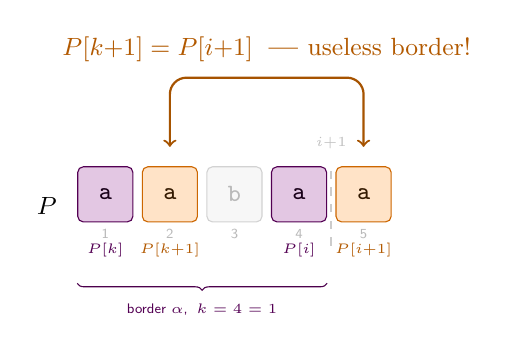
\begin{tikzpicture}[
  cell/.style={
    minimum width=7mm, minimum height=7mm,
    font=\ttfamily\small, inner sep=0pt,
    text centered, rounded corners=2pt,
  },
  Brd/.style={cell, draw=violet!65!black, fill=violet!22, text=violet!20!black},
  Nxt/.style={cell, draw=orange!80!black, fill=orange!22, text=orange!20!black},
  NC/.style ={cell, draw=gray!35,         fill=gray!6,    text=gray!55},
]
\def\cw{0.82}

% position indices
\foreach \i in {1,...,5}
  \node[font=\tiny\sffamily, text=gray!55] at ({(\i-1)*\cw}, 0.55) {\i};

% P label
\node[font=\small\ttfamily, anchor=east] at (-0.6*\cw, 0.9) {$P$};
\node[Brd] (p1) at (0*\cw, 1.05) {a};   
\node[Nxt] (p2) at (1*\cw, 1.05) {a};   
\node[NC]  (p3) at (2*\cw, 1.05) {b};
\node[Brd] (p4) at (3*\cw, 1.05) {a};   
\node[Nxt] (p5) at (4*\cw, 1.05) {a};   

% dashed separator
\draw[gray!40, dashed, thick]
  (3.5*\cw, 0.4) -- (3.5*\cw, 1.4);
\node[font=\tiny\sffamily, text=gray!50] at (3.5*\cw, 1.5)
  [above] {$i{+}1$};

% labels below
\node[font=\tiny\sffamily, text=violet!65!black, below=4pt] at (p1.south)
  {$P\kern0pt[k]$};
\node[font=\tiny\sffamily, text=orange!70!black, below=4pt] at (p2.south)
  {$P[k{+}1]$};
\node[font=\tiny\sffamily, text=violet!65!black, below=4pt] at (p4.south)
  {$P\kern0pt[i]$};
\node[font=\tiny\sffamily, text=orange!70!black, below=4pt] at (p5.south)
  {$P[i{+}1]$};

% curved arrow above
\draw[orange!65!black, thick, <->, rounded corners=6pt,
      shorten >=2pt, shorten <=2pt]
  ([yshift=5pt]p2.north) -- ([yshift=32pt]p2.north) --
  node[above=2pt, font=\small, text=orange!70!black]
    {$P[k{+}1] = P[i{+}1]$ \;\textbf{---} useless border!}
  ([yshift=32pt]p5.north) -- ([yshift=5pt]p5.north);

% brace under border
\draw[violet!60!black, decorate, decoration={brace, mirror, raise=22pt}]
  (p1.south west) -- (p4.south east)
  node[midway, below=26pt, font=\tiny\sffamily, text=violet!65!black]
    {border $\alpha$, \;$k = \spi{4} = 1$};

\end{tikzpicture}
\caption{%
  Strong border for $P = \texttt{aabaa}$ at $i=4$.
  The border $\alpha = \texttt{a}$ (\textcolor{violet!65!black}{violet},
  $k=\spi{4}=1$) satisfies $P\kern0pt[1]=P\kern0pt[4]$,
  but its ``next character'' $P[k{+}1]=P\kern0pt[2]=\texttt{a}$
  (\textcolor{orange!70!black}{orange}) equals $P[i{+}1]=P\kern0pt[5]=\texttt{a}$.
  Any mismatch on $P\kern0pt[5]$ with text character $x\neq\texttt{a}$ would
  \emph{also} fail immediately at $P[k{+}1]$ after the fallback ---
  the border is useless.
  Hence $\spi{4}'=0$: skip straight to the start.
}
\label{fig:strong-border}
\end{figure}

$\spi{i}'$ skips the entire chain of useless borders in one step, but it only encodes a
single fallback state --- the longest ``safe'' border for the specific character $P[i+1]$.
For a completely arbitrary text character $x$, a fallback chain might still occur. To achieve 
strict $\Oh{1}$ time per character, a full character-indexed table is needed.

\subsubsection{Character-indexed borders and the DFA: True Real-Time}

For a complete real-time solution we precompute, for each position $i$ and character
$x \in \Sigma$, the longest border of $P[1\ldots i]$ whose next character is exactly $x$:

\begin{definition}[$sp_{i,x}$ values]
  For $i \in \{0,1,\ldots,m\}$ and $x \in \Sigma$,
  \[
    \mathrm{sp}_{i,x}(P) \;=\; \max\bigl\{\, k \leq \spi{i} \mid P[k+1] = x \,\bigr\},
  \]
  with default $0$ when no such $k$ exists.
\end{definition}

This generalises $\spi{i}'$: where the strong border encodes a single fallback state for the
character $P[i+1]$, the table $\mathrm{sp}_{i,x}$ encodes the optimal fallback for \emph{every}
$x \in \Sigma$ simultaneously.

\begin{example}[$sp'$ vs.\ $\mathrm{sp}_{i,x}$ for $P = \texttt{aabaab}$]
\label{ex:sp-vs-spix}
Consider $P = \texttt{aabaab}$ ($m=6$) over $\Sigma=\{\texttt{a},\texttt{b},\texttt{c}\}$.
The $sp$ and $sp'$ values are:

\begin{center}
\begin{tabular}{rcccccc}
  \toprule
  $i$            & 1 & 2 & 3 & 4 & 5 & 6 \\
  \midrule
  $P[i]$         & \texttt{a} & \texttt{a} & \texttt{b} & \texttt{a} & \texttt{a} & \texttt{b} \\
  $\spi{i}$      & 0 & 1 & 0 & 1 & 2 & 3 \\
  $\spi{i}'$     & 0 & 1 & 0 & 0 & 1 & -- \\
  \bottomrule
\end{tabular}
\end{center}

\aside{%
  At $i=5$, the border chain of $P[1..5]=\texttt{aabaa}$ is
  $k \in \{2,\,1,\,0\}$.
  Both $k=2$ ($P[3]{=}\texttt{b}{=}P[6]$) and $k=1$ ($P[2]{=}\texttt{a}$)
  must be inspected; $\spi{5}'=1$ skips past the useless $k=2$.}
At $i=5$ the border $\texttt{aa}$ ($\spi{5}=2$) is useless because $P[3]=\texttt{b}=P[6]$;
the shorter border $\texttt{a}$ ($k=1$) satisfies $P[2]=\texttt{a}\neq P[6]$, so
$\spi{5}'=1$.

Now suppose we have matched $P[1..5]$ (state $j=5$) and the next text character is $x$.
With $\spi{5}'=1$, KMP falls back to state~$1$ for \emph{every} mismatch
$x \neq P[6]=\texttt{b}$, and may still need further comparisons depending on $x$:

\aside[-2ex]{%
  $\mathrm{sp}_{5,\texttt{a}}=1$ because the border of length~$1$
  satisfies $P[2]=\texttt{a}=x$; no border has $P[k{+}1]=\texttt{c}$,
  so $\mathrm{sp}_{5,\texttt{c}}=0$.}
\begin{itemize}[topsep=4pt, itemsep=3pt]
  \item $x=\texttt{a}$: $5\to 1$, then $P[2]=\texttt{a}=x \Rightarrow$ state $2$.
        \textbf{Two comparisons.}
  \item $x=\texttt{c}$: $5\to 1$, $P[2]\neq\texttt{c}$; $1\to 0$, $P[1]\neq\texttt{c}$;
        stay at $0$. \textbf{Three comparisons.}
\end{itemize}
By contrast, $\mathrm{sp}_{5,x}$ resolves every case in one lookup:

\begin{center}
\begin{tabular}{rccc}
  \toprule
  $x$                      & \texttt{a} & \texttt{b} & \texttt{c} \\
  \midrule
  $\mathrm{sp}_{5,x}$     & 1 & -- \textnormal{\scriptsize (match $P[6]$)} & 0 \\[3pt]
  DFA $\delta(5,x)$        & 2 & 6 \textnormal{\scriptsize (full match!)}   & 0 \\
  \bottomrule
\end{tabular}
\end{center}

$\delta(5,\texttt{a})=2$ replaces two comparisons with one table read;
$\delta(5,\texttt{c})=0$ replaces three.
\end{example}

The table $\{\mathrm{sp}_{i,x}(P)\}_{i,x}$ is precisely the \emph{transition function} of
the deterministic finite automaton (DFA)\aside[1ex]{%
  The DFA has $m+1$ states and $|\Sigma|$ transitions per state, so the table takes
  $\Oh{m|\Sigma|}$ space and time to build.} for pattern $P$: state $i$ encodes ``$i$ characters
of $P$ matched so far'', and on reading $x$ the automaton transitions to
$\mathrm{sp}_{i,x}(P) + \mathbf{1}[P[i+1]=x]$.
With this table, each character of $T$ is processed in strict $\Oh{1}$ worst-case time, making
KMP truly \textbf{real-time}.


% ══════════════════════════════════════════════════════════════════
\subsection{A Comprehensive Trace: KMP and Z-Algorithm}
% ══════════════════════════════════════════════════════════════════

To solidify these concepts, let's trace KMP and then contrast it directly with the Z-Algorithm.

\subsubsection{KMP Step-by-Step}

Consider the pattern $P = \texttt{ababa}$ and the text $T = \texttt{ababcababa}$.
Here we trace the standard KMP behavior (using plain $sp$ values to illustrate the fallback mechanism that DFA optimizes).\aside[2ex]{For $i=4$, $P[1..4]=\texttt{abab}$. Proper prefix-suffixes are $\texttt{ab}$ (len 2) and $\texttt{a}$ (len 1). Max is 2.}

\paragraph{1. Preprocessing $P$.}
We compute the $sp$ array for $P$.
\begin{center}
\begin{tabular}{rccccc}
  \toprule
  $i$    & 1 & 2 & 3 & 4 & 5 \\
  \midrule
  $P\kern0pt[i]$ & \texttt{a} & \texttt{b} & \texttt{a} & \texttt{b} & \texttt{a} \\
  $\spi{i}$ & 0 & 0 & 1 & 2 & 3 \\
  \bottomrule
\end{tabular}
\end{center}

\paragraph{2. Searching $T$.}
We maintain a pointer $i$ into $T$ and a pointer $j$ representing the length of the current match in $P$.
The complete trace is shown in Figure~\ref{fig:kmp-trace}.

% ── Figure: KMP Full Trace ────────────────────────────────
\begin{figure}[H]
\centering
\begin{tikzpicture}[
  cell/.style={
    minimum width=6.5mm, minimum height=6.5mm,
    font=\ttfamily\small, inner sep=0pt,
    text centered, rounded corners=2pt,
  },
  Tcell/.style={cell, draw=blue!50!black, fill=blue!8},
  Match/.style={cell, draw=green!55!black, fill=green!18, text=green!30!black},
  Fail/.style ={cell, draw=red!65!black,   fill=red!12,   text=red!50!black},
  Skip/.style ={cell, draw=gray!30,        fill=gray!5,    text=gray!40},
  Pointer/.style={-Stealth, thick, red!70!black},
]
\def\cw{0.75}

% --- Text T ---
\node[font=\small\ttfamily, anchor=east] at (-0.5, 3.5) {$T$};
\foreach \i/\c in {1/a, 2/b, 3/a, 4/b, 5/c, 6/a, 7/b, 8/a, 9/b, 10/a}
  \node[Tcell] (t\i) at ({(\i-1)*\cw}, 3.5) {\c};

% --- Step 1: i=1 to 4, match abab ---
\node[font=\tiny\sffamily, text=gray] at (-0.7, 2.5) {Step 1};
\foreach \i/\c in {1/a, 2/b, 3/a, 4/b} \node[Match] at ({(\i-1)*\cw}, 2.5) {\c};
\node[Fail] at (4*\cw, 2.5) {a}; % P\kern0pt[5]
\node[font=\tiny\sffamily, text=red!70!black, anchor=west] at (10.5*\cw, 2.5) {$T\kern0pt[5]=\texttt{c} \neq P\kern0pt[5]$};

% --- Fallback ---
\draw[Pointer] (4*\cw, 2.2) -- (4*\cw, 1.8);
\node[font=\tiny\sffamily, text=red!70!black, anchor=west] at (10.5*\cw, 2.0) {mismatch! $j \gets sp\kern0pt[4]=2$};

% --- Step 2: i=5, match aba? No ---
\node[font=\tiny\sffamily, text=gray] at (-0.7, 1.5) {Step 2};
\node[Skip] at (2*\cw, 1.5) {a}; \node[Skip] at (3*\cw, 1.5) {b}; % aligned ab
\node[Fail] at (4*\cw, 1.5) {a}; % P\kern0pt[3]
\node[font=\tiny\sffamily, text=red!70!black, anchor=west] at (10.5*\cw, 1.5) {$T\kern0pt[5]=\texttt{c} \neq P\kern0pt[3]$};

% --- Fallback ---
\draw[Pointer] (4*\cw, 1.2) -- (4*\cw, 0.8);
\node[font=\tiny\sffamily, text=violet!80!black, anchor=west] at (10.5*\cw, 1.0) {$j \gets sp\kern0pt[2]=0$};

% --- Step 3: i=5, match a? No ---
\node[font=\tiny\sffamily, text=gray] at (-0.7, 0.5) {Step 3};
\node[Fail] at (4*\cw, 0.5) {a}; % P\kern0pt[1]
\node[font=\tiny\sffamily, text=red!70!black, anchor=west] at (10.5*\cw, 0.5) {$T\kern0pt[5]=\texttt{c} \neq P\kern0pt[1]$};

% --- Step 4: i=6 to 10, Match! ---
\node[font=\tiny\sffamily, text=gray] at (-0.7, -0.5) {Step 4};
\foreach \i/\c [evaluate=\i as \tx using int(\i+5)] in {1/a, 2/b, 3/a, 4/b, 5/a}
  \node[Match] at ({(\tx-1)*\cw}, -0.5) {\c};
\node[font=\tiny\bfseries\sffamily, text=green!45!black, anchor=west] at (10.5*\cw, -0.5) {MATCH!};

\end{tikzpicture}
\caption{KMP trace for $P=\texttt{ababa}$ in $T=\texttt{ababcababa}$. Step 1 finds a mismatch at $T\kern0pt[5]$. KMP falls back twice ($j=4 \to 2 \to 0$) without re-reading $T$. Finally, Step 4 finds a complete match starting at $T\kern0pt[6]$.}
\label{fig:kmp-trace}
\end{figure}

\subsubsection{Online vs.\ Real-Time: Bridging the Gap}

The KMP trace above highlights a crucial property: KMP processes $T$ one character at a time without ever stepping backwards in $T$. This makes KMP an \textbf{online} algorithm. However, as seen in Steps 1-3, processing the single character $T[5]=\texttt{c}$ required multiple internal operations ($j$ falling back multiple times). If we had used the full DFA ($\mathrm{sp}_{i,x}$) discussed previously, those steps would collapse into $\Oh{1}$ worst-case time, upgrading the algorithm from merely online to strictly \textbf{real-time}.

By contrast, the Z-algorithm is \emph{neither} real-time nor strictly online in the same way. The computation of the Z-box $[l,r]$ depends on reading characters ahead in the string. Let's trace it to see this structural difference in action.

\subsubsection{Z-Algorithm Trace}

Let's compute the Z-values for the string $S = \texttt{aababca}$. 
Notice how the algorithm looks ahead to establish the rightmost boundary $r$.

\begin{enumerate}
  \item \textbf{$i=2$:} $S[2]=\texttt{a} = S[1]$. Check $S[3]=\texttt{b} \neq S[2]$. $Z_2 = 1$.
        Box $[l,r] = [2,2]$.
  \item \textbf{$i=3$:} $i > r=2$. $S[3]=\texttt{b} \neq S[1]$. $Z_3 = 0$. Box stays $[2,2]$.
  \item \textbf{$i=4$:} $i > r=2$. $S[4]=\texttt{a} = S[1]$. Check $S[5]=\texttt{b} = S[2]$, $S[6]=\texttt{c} \neq S[3]$. $Z_4 = 2$.
        New box $[l,r] = [4,5]$.
  \item \textbf{$i=5$:} $i \leq r=5$. Mirror $k = i-l+1 = 5-4+1 = 2$.
        $Z_k = Z_2 = 1$. Remaining box width $r-i+1 = 5-5+1 = 1$.
        Since $Z_k \not< r-i+1$ (Case 2b), we try to extend from $r+1 = 6$.
        $S[6]=\texttt{c} \neq S[3]$. No extension. $Z_5 = 1 + 0 = 1$. Box stays $[4,5]$.
  \item \textbf{$i=6$:} $i > r=5$. $S[6]=\texttt{c} \neq S[1]$. $Z_6 = 0$.
  \item \textbf{$i=7$:} $i > r=5$. $S[7]=\texttt{a} = S[1]$. No more chars. $Z_7 = 1$.
\end{enumerate}

\begin{center}
\begin{tabular}{rccccccc}
  \toprule
  $i$    & 1 & 2 & 3 & 4 & 5 & 6 & 7 \\
  \midrule
  $S[i]$ & \texttt{a} & \texttt{a} & \texttt{b} & \texttt{a} & \texttt{b} & \texttt{c} & \texttt{a} \\
  $Z_i$  & -- & 1 & 0 & 2 & 1 & 0 & 1 \\
  \bottomrule
\end{tabular}
\end{center}


\subsection{Boyer-Moore Algorithm}
So far we have seen two algorithms that scan the text from left to right, never re-reading
any character of $T$ once processed. Is this mandatory? Or can we change this approach?

The Boyer-Moore algorithm scans the text from right to left, starting with the last character of
the pattern aligned with the current text position. Why would this be a good idea?

In this algorithm checks are computed from right to left, while the pattern is aligned with the text from left to right. 

What are the advantages of this approach? Let's consider the following heuristics:
\begin{itemize}
  \item \textbf{Bad Character Rule}: during preprocessing, for each position $i$ and character $x$, we keep memory of the first occurrence of $x$ to the left of $i$.
  
  \begin{center}
  \begin{tikzpicture}[
    cell/.style={minimum width=7mm, minimum height=7mm, font=\ttfamily\small, inner sep=0pt, text centered, rounded corners=2pt},
    Tcell/.style={cell, draw=blue!50!black, fill=blue!8},
    XC/.style={cell, draw=red!65!black, fill=red!12, text=red!50!black},
  ]
    \draw[blue!50!black, fill=blue!8, rounded corners=2pt] (0,0) rectangle (5, 0.4);
    \draw[thick, red!70!black] (3.5, 0) -- (3.5, 0.4) node[above, font=\small\sffamily] {$i$};
    \draw[thick, orange!80!black] (2.5, 0) -- (2.5, 0.4) node[above, font=\small\sffamily] {$x$};
    \draw[<-, thick, Stealth-, bend right=45] (2.6, -0.2) to (3.4, -0.2);
    \node[below, font=\tiny\sffamily, text=gray!80] at (3, -0.5) {shift to align $x$};
  \end{tikzpicture}
  \end{center}

  \item \textbf{Good Suffix Rule}: during preprocessing, for each suffix of $P$, we keep memory of its first further occurrence to the left.
  
  \begin{center}
  \begin{tikzpicture}[
    cell/.style={minimum width=7mm, minimum height=7mm, font=\ttfamily\small, inner sep=0pt, text centered, rounded corners=2pt},
    Tcell/.style={cell, draw=blue!50!black, fill=blue!8},
    Alpha/.style={cell, draw=violet!70!black, fill=violet!25, text=violet!20!black},
  ]
    \draw[blue!50!black, fill=blue!8, rounded corners=2pt] (0,0) rectangle (5, 0.4);
    \draw[violet!70!black, fill=violet!25, rounded corners=2pt] (3.3, 0) rectangle (5, 0.4) node[midway, font=\tiny\sffamily] {suffix};
    \draw[violet!70!black, fill=violet!25, rounded corners=2pt] (1, 0) rectangle (2.7, 0.4) node[midway, font=\tiny\sffamily] {copy};
    \draw[<-, thick, Stealth-, bend left=45] (1.85, 0.6) to (4.15, 0.6);
  \end{tikzpicture}
  \end{center}
\end{itemize}
